\documentclass[a4paper, 11pt]{article}
\usepackage[ngerman]{babel}
%ä und so
\usepackage[utf8]{inputenc}
\usepackage[T1]{fontenc}
\usepackage{amsmath}
\usepackage{amsthm}
\usepackage{amsbsy}

\usepackage{mathrsfs}
\usepackage{amssymb}
\usepackage{amstext}
\usepackage{amsfonts}
\usepackage{float}
\usepackage{graphicx}
\usepackage{esdiff}
\usepackage{hyperref}
\usepackage{geometry}
\geometry{top = 20mm, bottom = 20 mm, left = 25mm, right = 25mm}


\usepackage{setspace}
\onehalfspacing

\usepackage{fancyhdr}
\usepackage{wrapfig}
%\usepackage[hyphens]{url}
%\urlstyle{sf}
%\usepackage[hidelinks]{hyperref}
%\usepackage{breakurl}
%\hypersetup{colorlinks=false}
\usepackage{multirow}
\usepackage[bottom]{footmisc}

%\usepackage{svg}

\title{Optik II - Michelson-Interferometer}
\author{Gruppe B14 \\ \\ Daniel Wendland \\ Philipp Bremer \\ Olexiy Fedorets \\ Jonathan Hermann}
\date{\today}

% !TeX spellcheck = de_DE
\begin{document}


\begin{titlepage}
	\vspace*{\fill}
	\begin{center}
		\vskip -0.25\textheight
		\vfill
		\newcommand{\Line}{\rule{\linewidth}{0.6mm}}
		\Line 
		{\let\newpage\relax\maketitle}
		\Line 
		\vfill
	\end{center}

	
	\vspace*{\fill}
	\thispagestyle{empty}
\end{titlepage}





\newpage
\thispagestyle{empty}
\tableofcontents
\newpage

%Kopf- und Fußzeile
\pagestyle{fancy}
\fancyhf{}
%Kopfzeile links bzw. innen
\fancyhead[L]{\nouppercase{\leftmark}}
%Kopfzeile rechts bzw. außen
\fancyhead[R]{\thepage}
%Linie oben
\renewcommand{\headrulewidth}{0.5pt}
\fancyfoot[C]{\thepage}


\setcounter{page}{1}

\section{Einleitung}
Dieser Versuch beschäftigt sich mit dem Michelson-Interferometer und hat als Ziel die Charakterisierung eines grünen Lasers anhand seiner Wellenlänge. Weiterhin soll noch die Druckabhängigkeit des Brechungsindex von Luft untersucht und dann der Brechungsindex von $\mathrm{CO_2}$ bestimmt werden.


\section{Messung der Wellenlänge}

\subsection{Aufbau und Grundlagen} 

\begin{figure}[H]
	\centering
	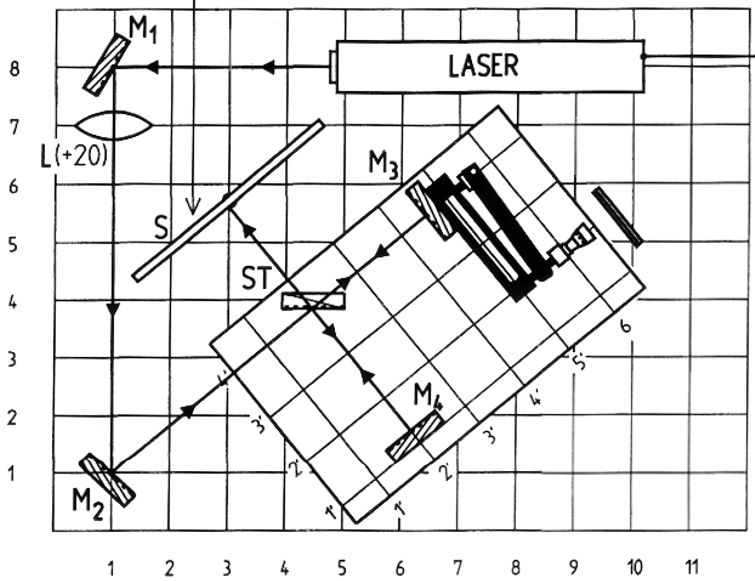
\includegraphics[trim = 0mm 0mm 0mm 0mm,clip, width=12cm]{Bilder/aufbau_optik2.png}%
	\caption[Strahlengang im Aufbau]{Strahlengang im Aufbau}%
	\label{pic:Abbildung 1}%
\end{figure}

\begin{figure}[H]
	\centering
	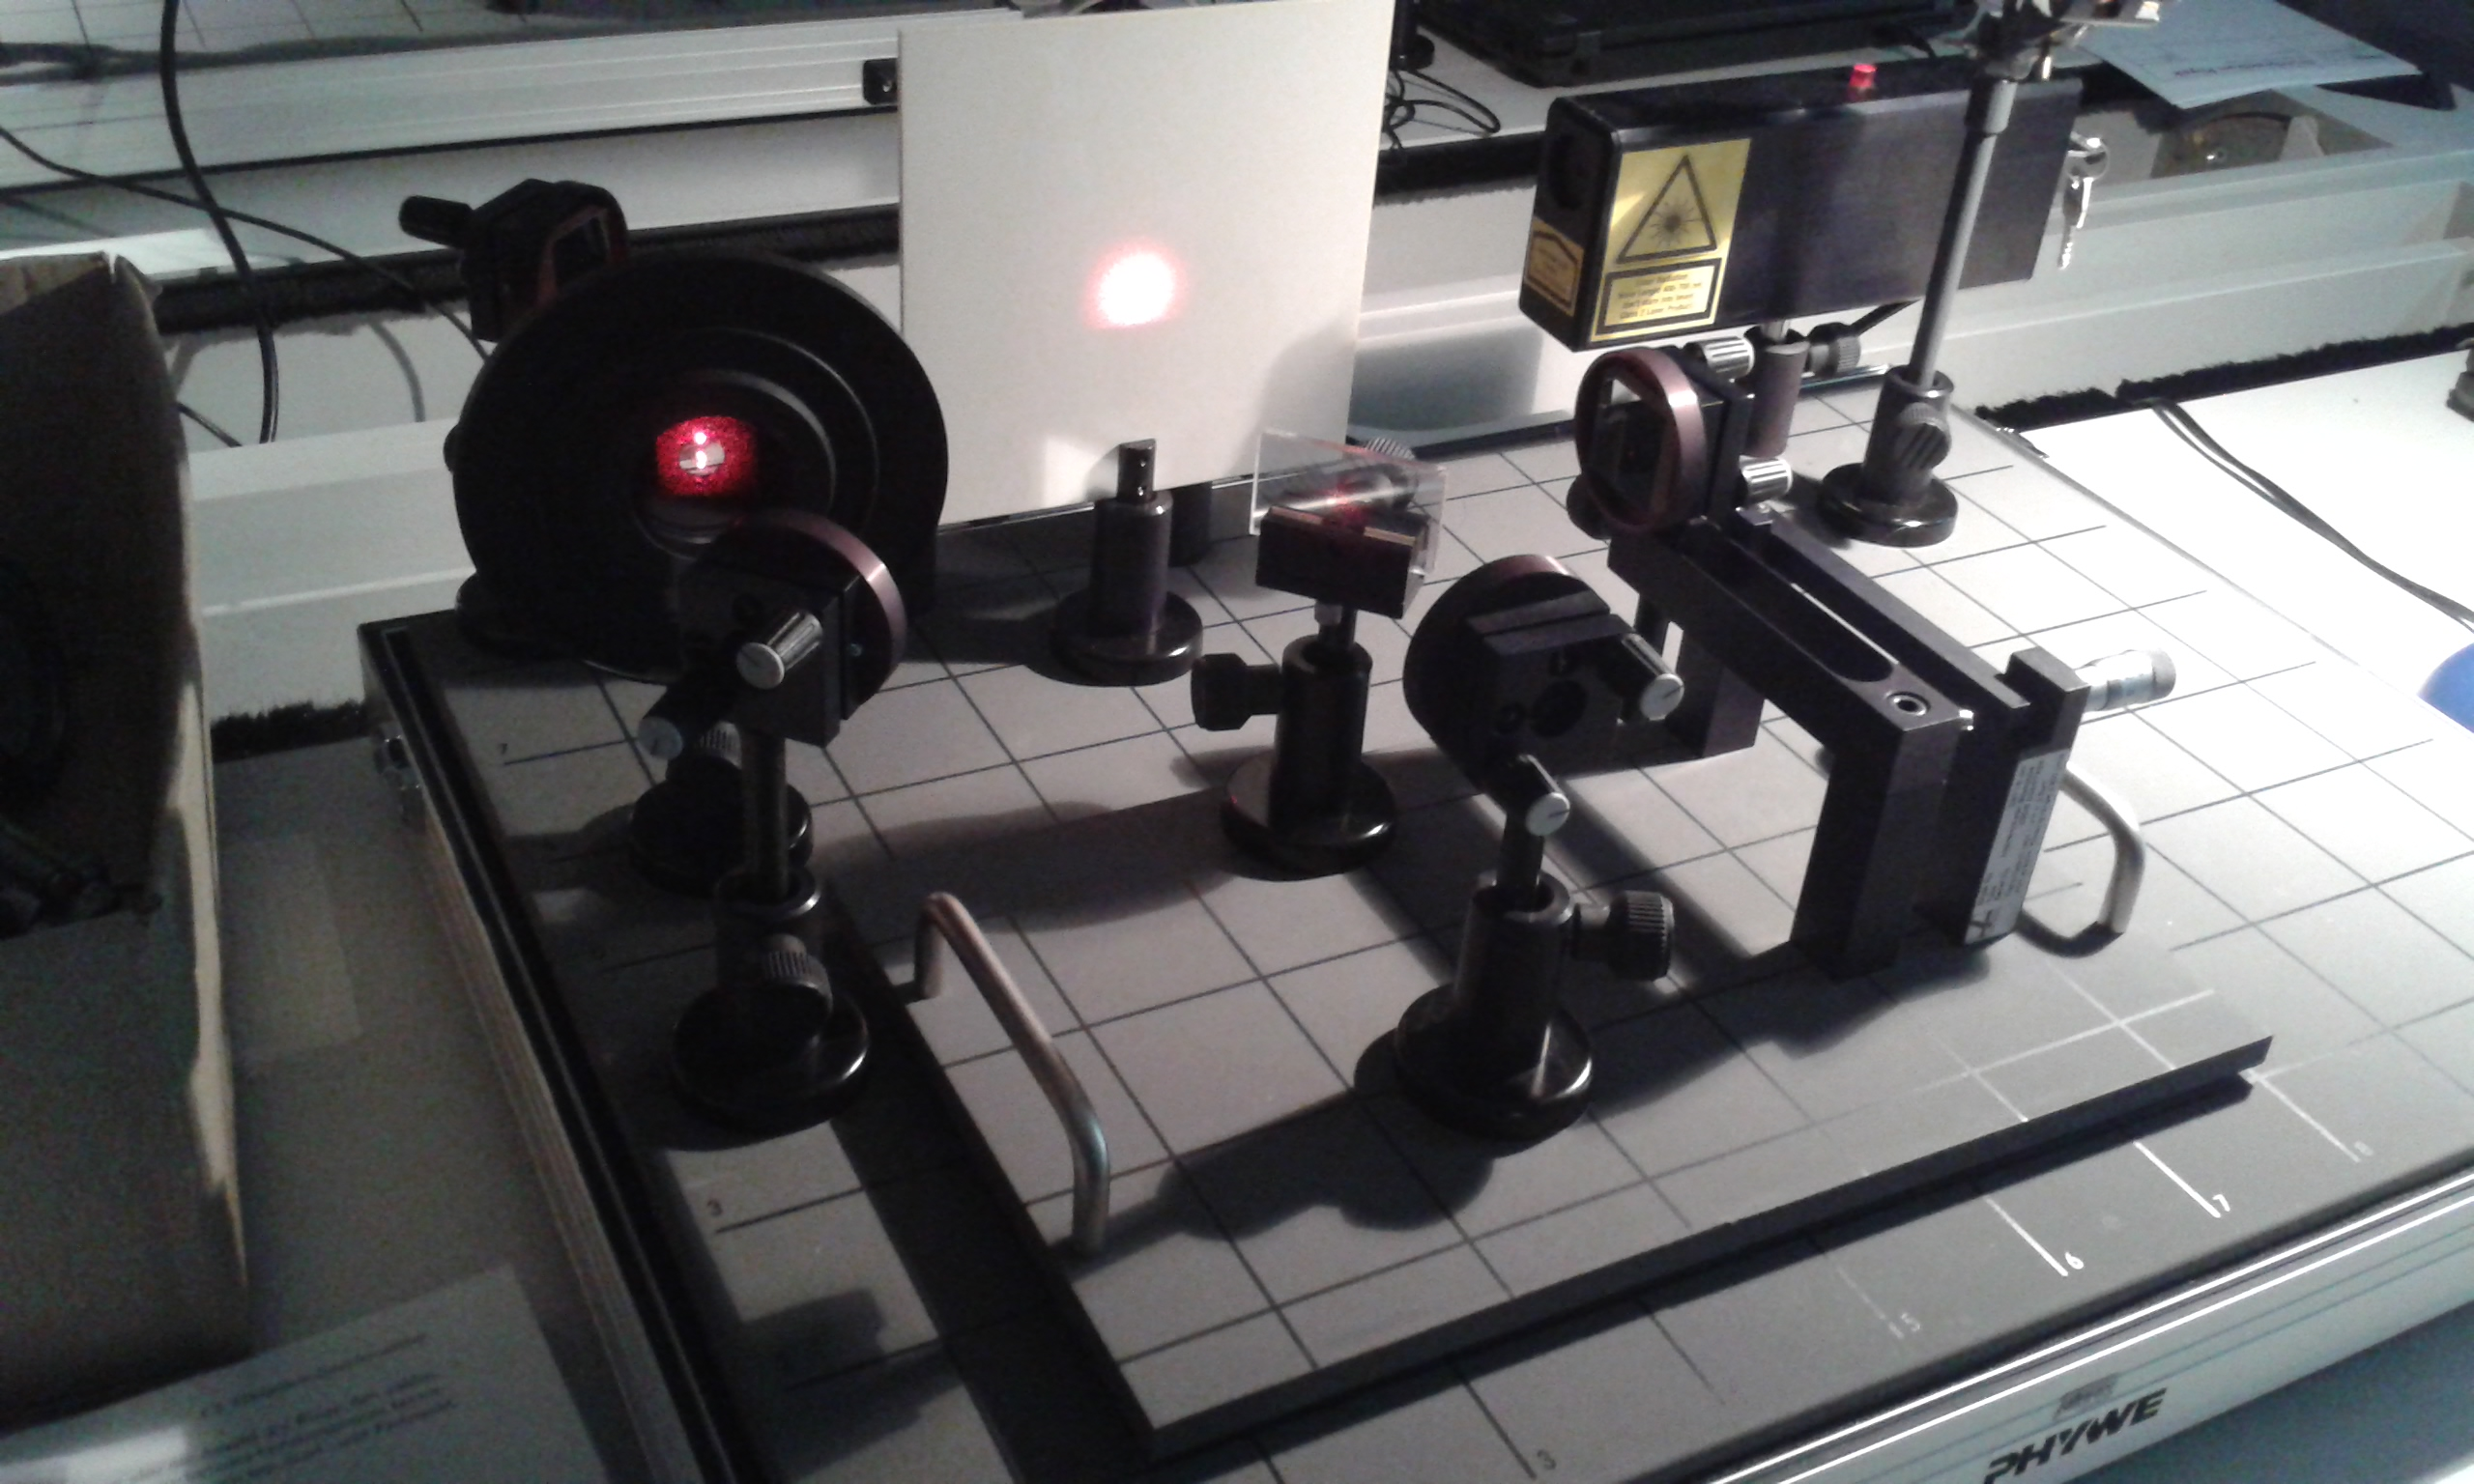
\includegraphics[scale=0.25]{Bilder/Aufbau.jpg}%
	\caption{Aufgebautes Michelson-Interferometer}%
	\label{pic:Michelson}%
\end{figure}

Das Michelson-Interferometer wird auf einer magnetischen Platte aufgebaut, auf der die einzelnen Komponenten, mit Stativen die in magnetischen Füßen stecken, relativ fest installiert werden können.
Aus Platzgründen wird der Laserstrahl, bevor er auf den Strahlteiler und damit den Hauptteil des Versuchs trifft, zweifach umgelenkt (hier durch M1 und M2). Damit der Strahl nach Kontakt mit dem Strahlteiler in Richtung M3 und M4 abgelenkt wird, wird der Strahlteiler so ausgerichtet das der Strahl in einem Winkel von $45^\circ$ zum Flächenlot einfällt. Die Spiegel M3 und M4 werden so ausgerichtet das der von ihnen reflektierte Strahl der in Richtung Laser geht, genau in die Austrittsöffnung des Lasers trifft. Nun sollte auf dem Schirm bereits ein Punkt zu sehen sein, der Interferenzerscheinungen zeigt, sobald an der Mikrometerschraube gedreht wird. Um ein größeres, besser zu erkennendes Interferenzbild zu erhalten wird zwischen M1 und M2 eine Streulinse eingebaut um den Strahl aufzuweiten, so dass nun auf dem Schirm Interferenzringe zu erkenne sein sollten. Dabei wurde von Gruppe 1 der 3. Aufbau und von Gruppe 2 der 4. Aufbau verwendet.


Das Prinzip eines Interferometers besteht darin das verschiedene Wellenzüge überlagert werden und mit einander interferieren. Damit Wellen überhaupt miteinander interferieren können müssen sie eine feste Phasenbeziehung haben, ihre Frequenz muss gleich sein und der Gangunterschied muss kleiner als die Kohärenzlänge sein. Um diese Bedingungen zu erfüllen wird beim Michelson-Interferometer ein Strahlteiler(ST) verwendet der den ursprünglichen Strahl zu $50\%$ transmittieren lässt und den Rest reflektiert.  Um nun die Strahlen wieder zusammenzuführen, treffen sie nach dem Teiler wieder auf Spiegel und werden durch ihn erneut abgelenkt. Dadurch wird ein Teil überlagert und auf dem Schirm abgebildet und der Rest zurück in den Laser gelenkt. Wenn nun der optische Weg zwischen Spiegel und Teiler nicht der gleiche ist, tritt auf Grund der optischen Wegdifferenz $ \Delta d = n \cdot \Delta x$ (mit geometrischer Wegdifferenz $\Delta x$) ein Gangunterschied am Schirm von $\Delta g=2 \cdot \Delta d $ auf. Da der Laserstrahl leicht divergent ist und somit einen Öffnungswinkel $\theta_{max}$ hat , erweitert sich der Gangunterschied um einen Faktor $\cos(\theta)$. In unserem Versuch werden jedoch nur die Interferenzen im innersten Ring betrachtet, sodass $\theta=0$ der Term also $2 \cdot \Delta d$ bleibt. Die Bedingung für konstruktive Interferenz ist wie immer $\Delta g=m \cdot \lambda $, damit ergibt sich 
\begin{equation}
\lambda = \frac{2 \cdot \Delta d}{\Delta m}
\end{equation}

\subsection{Kalibration}
Um die Wellenlänge eines unbekannten Lasers bestimmen zu können, muss man zunächst die Übersetzungskonstante $k$ zwischen der optischen Wegdifferenz $d$ und der Verdrehung des Mikrometerschraube $s$, mit der man die Verschiebung des Spiegels $M_3$ einstellt, bestimmen. Man nimmt dazu einen linearen Zusammenhang $d = k \cdot s$ an, wobei hier gilt, dass 
\begin{equation}
d = m \cdot \frac{\lambda}{2} \quad \Rightarrow \quad k \cdot s = m \cdot \frac{\lambda}{2}
\end{equation}  
mit der Anzahl $m$ der zusätzlichen bzw. verschwundenen Maxima und der Wellenlänge $\lambda$ einer bekannten Lichtquelle.

\subsubsection{Durchführung}
Zunächst wird die Kalibration mit dem roten Laser durchgeführt, dessen Wellenlänge von $\lambda = 632.8 nm$ sehr genau bekannt ist. Hierzu wird ein Teil des linearen Bereiches (Tabelle \ref{table:lin_Bereich}) der Mikrometerschraube zwischen etwa $7.5$mm und $9$mm ausgemessen, um die Linearität des Zusammenhangs zwischen $s$ und $d$ zu garantieren.
\begin{table}[H]
	\large
	\centering
	\begin{tabular}{|c|c|c|}
		\hline 	&	Bereichsanfang	&	Bereichsende	\\
		\hline	Gruppe 1	&	$ 7.5\mathrm{mm}$		&	$ 8.9\mathrm{mm}$ \\
		\hline  Gruppe 2	&	$ 8\mathrm{mm} $		&	$ 9\mathrm{mm}$ \\
		\hline
	\end{tabular}
	\caption{Für die Kalibration und Wellenlängenmessung linearisierte Bereiche beider Gruppen}
	\label{table:lin_Bereich}
\end{table}
Für die eigentliche Messung stellt man zunächst die Mikrometerschraube beim Anfangswert so ein, dass man ein zentrales Maximum oder Minimum deutlich erkennen kann. Dann wird an der Mikrometerschraube gedreht, bis insgesamt zehn Maxima bzw. Minima das Zentrum des Interferenzbildes durchlaufen haben und notiert das zugehörige $s$. Diesen Vorgang wiederholt man, bis das gewählte Bereichsende erreicht ist.

Die Messung zur Bestimmung der Wellenlänge funktioniert vollkommen analog, man ersetzt bloß vorher den roten Laser durch den grünen und überprüft gegebenenfalls die Justierung des Aufbaus. Dabei muss natürlich darauf geachtet werden, dass man mit der Mikrometerschraube innerhalb des linearen Bereichs bleibt, da sonst die Kalibration nicht mehr gewährleistet ist.

\subsubsection{Ergebnisse der Kalibration}
Um den linearen Zusammenhang zwischen der optischen Wegdifferenz $d$ und der Verdrehung der Mikrometerschraube $s$ zu überprüfen und insbesondere, um den Übersetzungsfaktor $k$ zu bestimmen führt man eine lineare Regression der Form 
\begin{equation*}
m \cdot a + b = s
\end{equation*} 
durch, wobei $ a = \frac{\lambda}{2 k} $.
Die gemessenen Werte für $s$ sind in Tabelle \ref{table:Kalibration_Roh} zusammengefasst, Abbildungen \ref{pic:Kalibration_1} und \ref{pic:Kalibration_2} zeigen die entsprechenden linearen Regressionen.

\begin{table}[H]
	\renewcommand{\arraystretch}{1.2}
	\centering
	\begin{tabular}{|c|c|c|}
		\hline  $m$	&	$s_{\mathrm{Gruppe 1}} [mm]$	&	$s_{\mathrm{Gruppe 2}} [mm]$	\\
		\hline	  0	&	$ 7.56 $		&	$ 8.00$ \\
		\hline   10	&	$ 7.63 $		&	$ 8.06$ \\
		\hline   20	&	$ 7.70 $		&	$ 8.12$ \\
		\hline   30	&	$ 7.77 $		&	$ 8.19$ \\
		\hline   40	&	$ 7.83 $		&	$ 8.25$ \\
		\hline   50	&	$ 7.89 $		&	$ 8.32$ \\
		\hline   60	&	$ 7.96 $		&	$ 8.39$ \\
		\hline   70	&	$ 8.02 $		&	$ 8.46$ \\
		\hline   80	&	$ 8.09 $		&	$ 8.53$ \\
		\hline   90 &	$ 8.16 $		&	$ 8.60$ \\
		\hline  100	&	$ 8.22 $		&	$ 8.67$ \\
		\hline  110	&	$ 8.29 $		&	$ 8.73$ \\
		\hline  120	&	$ 8.34 $		&	$ 8.81$ \\
		\hline  130	&	$ 8.41 $		&	$ 8.88$ \\
		\hline  140	&	$ 8.47 $		&	$ 8.95$ \\
		\hline  150	&	$ 8.55 $		&	$ 9.02$ \\
		\hline  160	&	$ 8.61 $		&	$ $ \\
		\hline  170	&	$ 8.67 $		&	$ $ \\
		\hline  180	&	$ 8.74 $		&	$ $ \\
		\hline  190	&	$ 8.80 $		&	$ $ \\
		\hline  200	&	$ 8.87 $		&	$ $ \\
		\hline
	\end{tabular}
	\caption{Messwerte für die Kalibration}
	\label{table:Kalibration_Roh}
\end{table}

\begin{figure}[H]
	\centering
	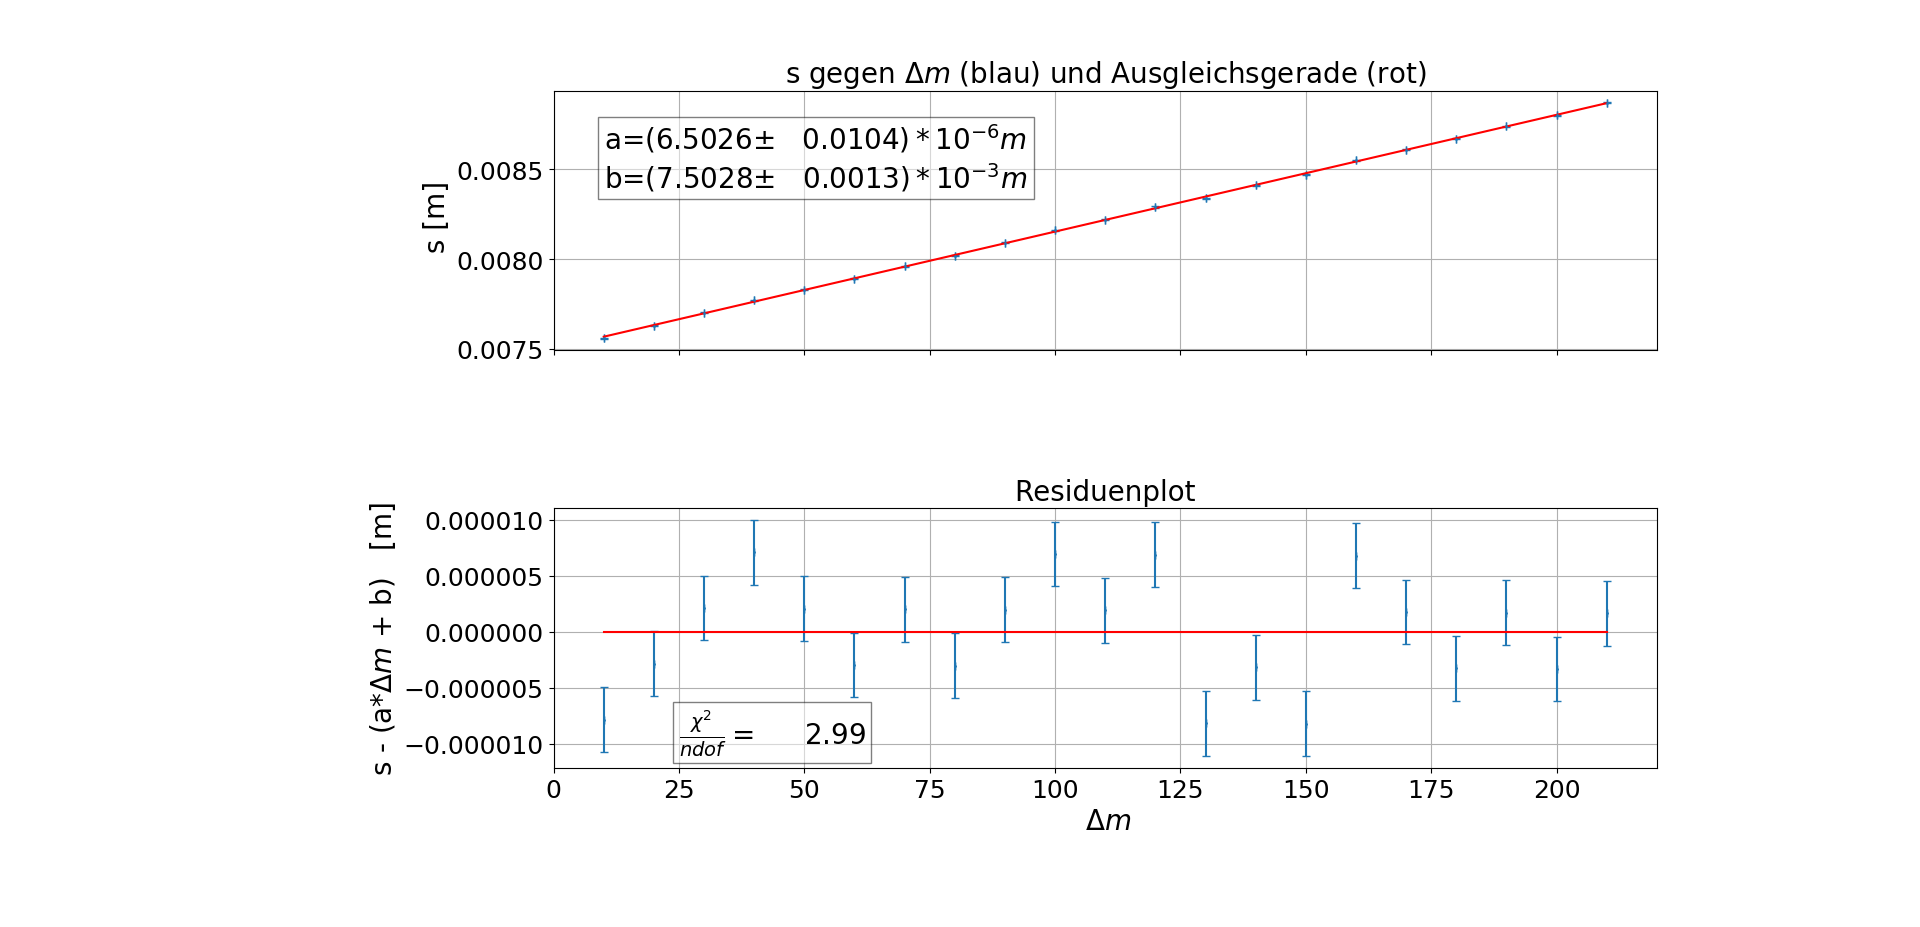
\includegraphics[trim={8cm 2cm 3cm 1cm},clip=true,width=1.1\linewidth]{./Bilder/Kalibration_1.png}
	\caption{Lineare Regression zur Kalibration - Gruppe 1}
	\label{pic:Kalibration_1}	
\end{figure}

\begin{figure}[H]
	\centering
	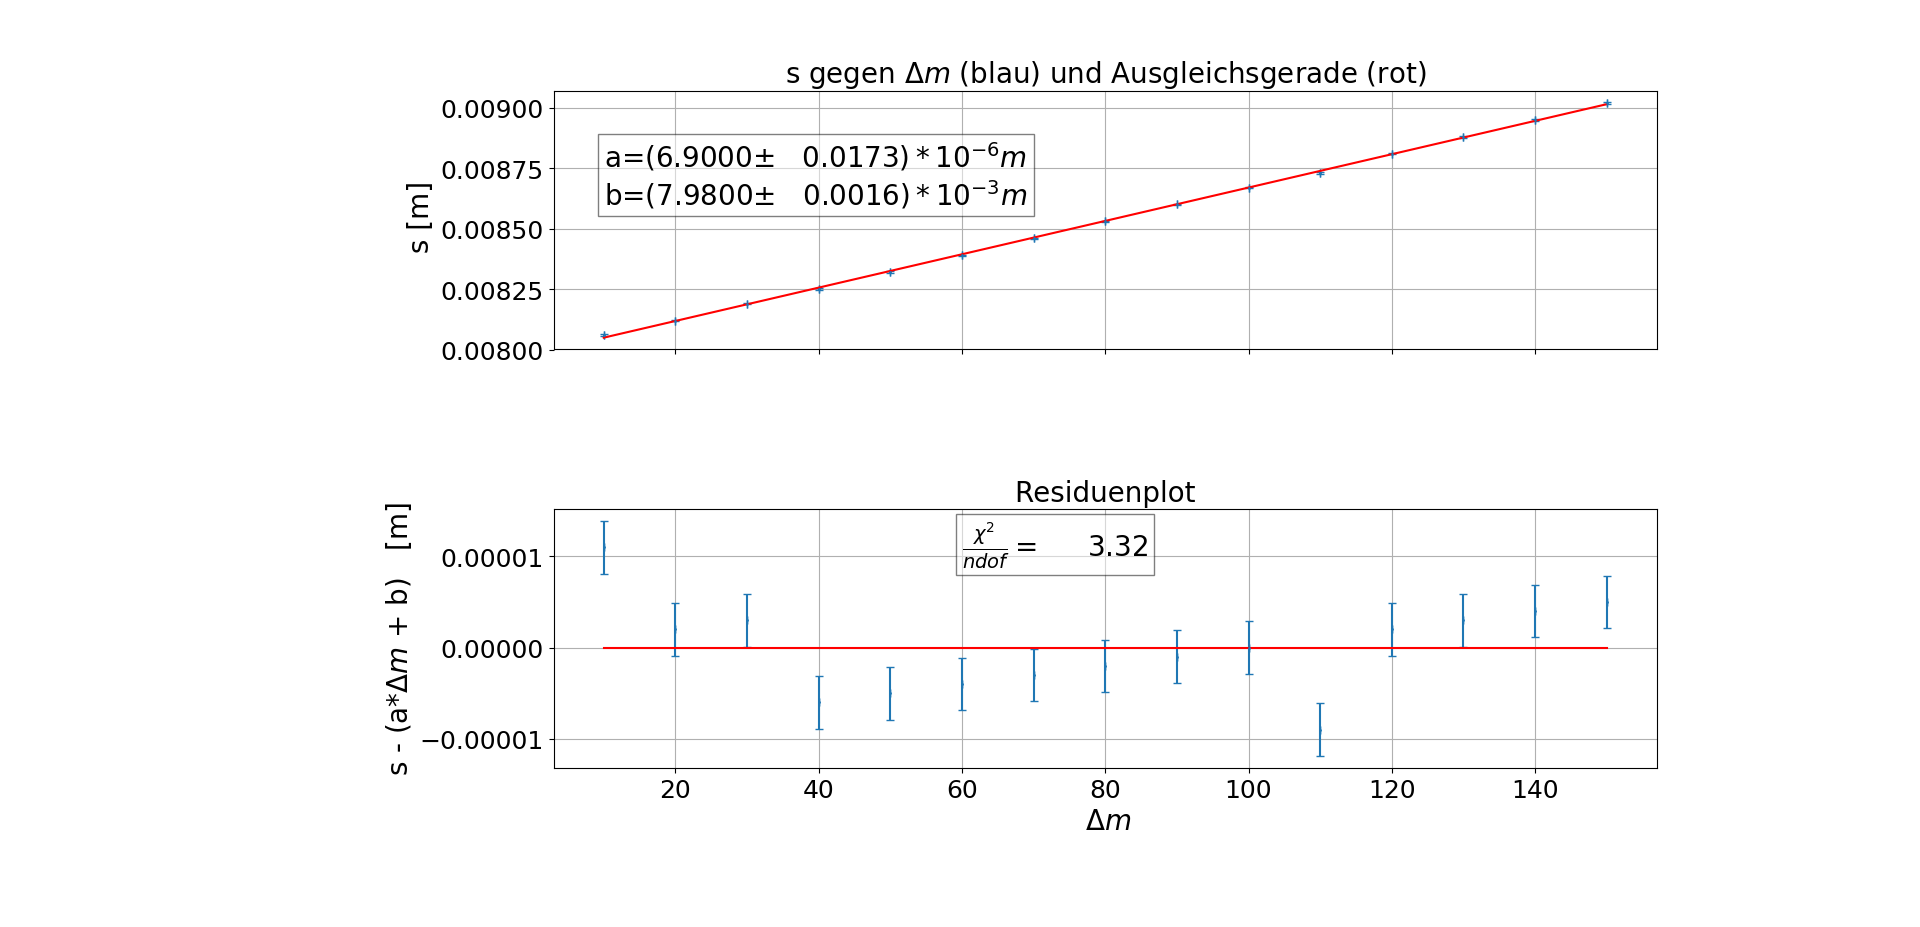
\includegraphics[trim={8cm 1cm 1cm 1cm},clip=true,width=1.1\linewidth]{./Bilder/Kalibration_2.png}
	\caption{Lineare Regression zur Kalibration - Gruppe 2}
	\label{pic:Kalibration_2}	
\end{figure}

Die Unsicherheit, die die Skalenwerte $s$ haben ergibt sich aus der Genauigkeit der Sklaeneinteilung auf der Mikrometerschraube von $10 \mu m$, so dass $\sigma_s = \frac{10 \mu m }{\sqrt{12}}$.
Aus der Steigung der linearen Regression kann man dann über $k = \frac{\lambda}{2a}$ auf $k$ schließen.
Die Unsicherheit auf a ergibt sich dann aus der gaußschen Fehlerfortpflanzung zu 
\begin{equation*}
\sigma_k = \frac{\lambda}{2a^2} \cdot \sigma_a
\end{equation*}
Die Unsicherheit auf die 
Wellenlänge kann vernachlässigt werden, da die relative Unsicherheit auf die Steigungen um einen Faktor 10 größer ist als die der Wellenlänge, denn die Wellenlänge von $632.8$nm ist auf weniger als $0.1$nm genau bestimmt. Die Ergebnisse der Kalibrationsmessung sind in Tabelle \ref{table:Kalibration} zusammengefasst. 
\begin{table}[H]
	\renewcommand{\arraystretch}{1.5}
	\centering
	\begin{tabular}{|c|c|c|}
		\hline  	&	Gruppe 1	&	Gruppe 2  	\\
		\hline	$a$ &	$ (6.503 \pm 0.010) \,\mu m$		&	$ (6.900 \pm 0.017)\, \mu m $ \\
		\hline  $b$	&	$ (7.5028 \pm 0.0013)\, mm$		&	$ (7.9800 \pm 0.0016)\, mm$ \\
		\hline  $k$	&	$ 0.04866 \pm 0.00008 $		&	$ 0.04586 \pm 0.00011$ \\
		\hline $\frac{\chi^2}{ndof}$	&	$2.99$	&	$3.32$	\\
		\hline
	\end{tabular}
	\caption{Ergebnisse der Kalibrationsmessung}
	\label{table:Kalibration}
\end{table}

\subsection{Auswertung}
Mit diesen Ergebnissen lässt sich nun die Wellenlänge des grünen Lasers bestimmen. Dazu führt man die gleiche lineare Regression der Form 
\begin{equation}
a \cdot m + b = s
\end{equation} mit Steigung $ a = \frac{\lambda}{2 k} $ an der Messreihe für den grünen Laser durch (siehe Abbildungen \ref{pic:lambda_1} und \ref{pic:lambda_2}).

\begin{figure}[H]
	\centering
	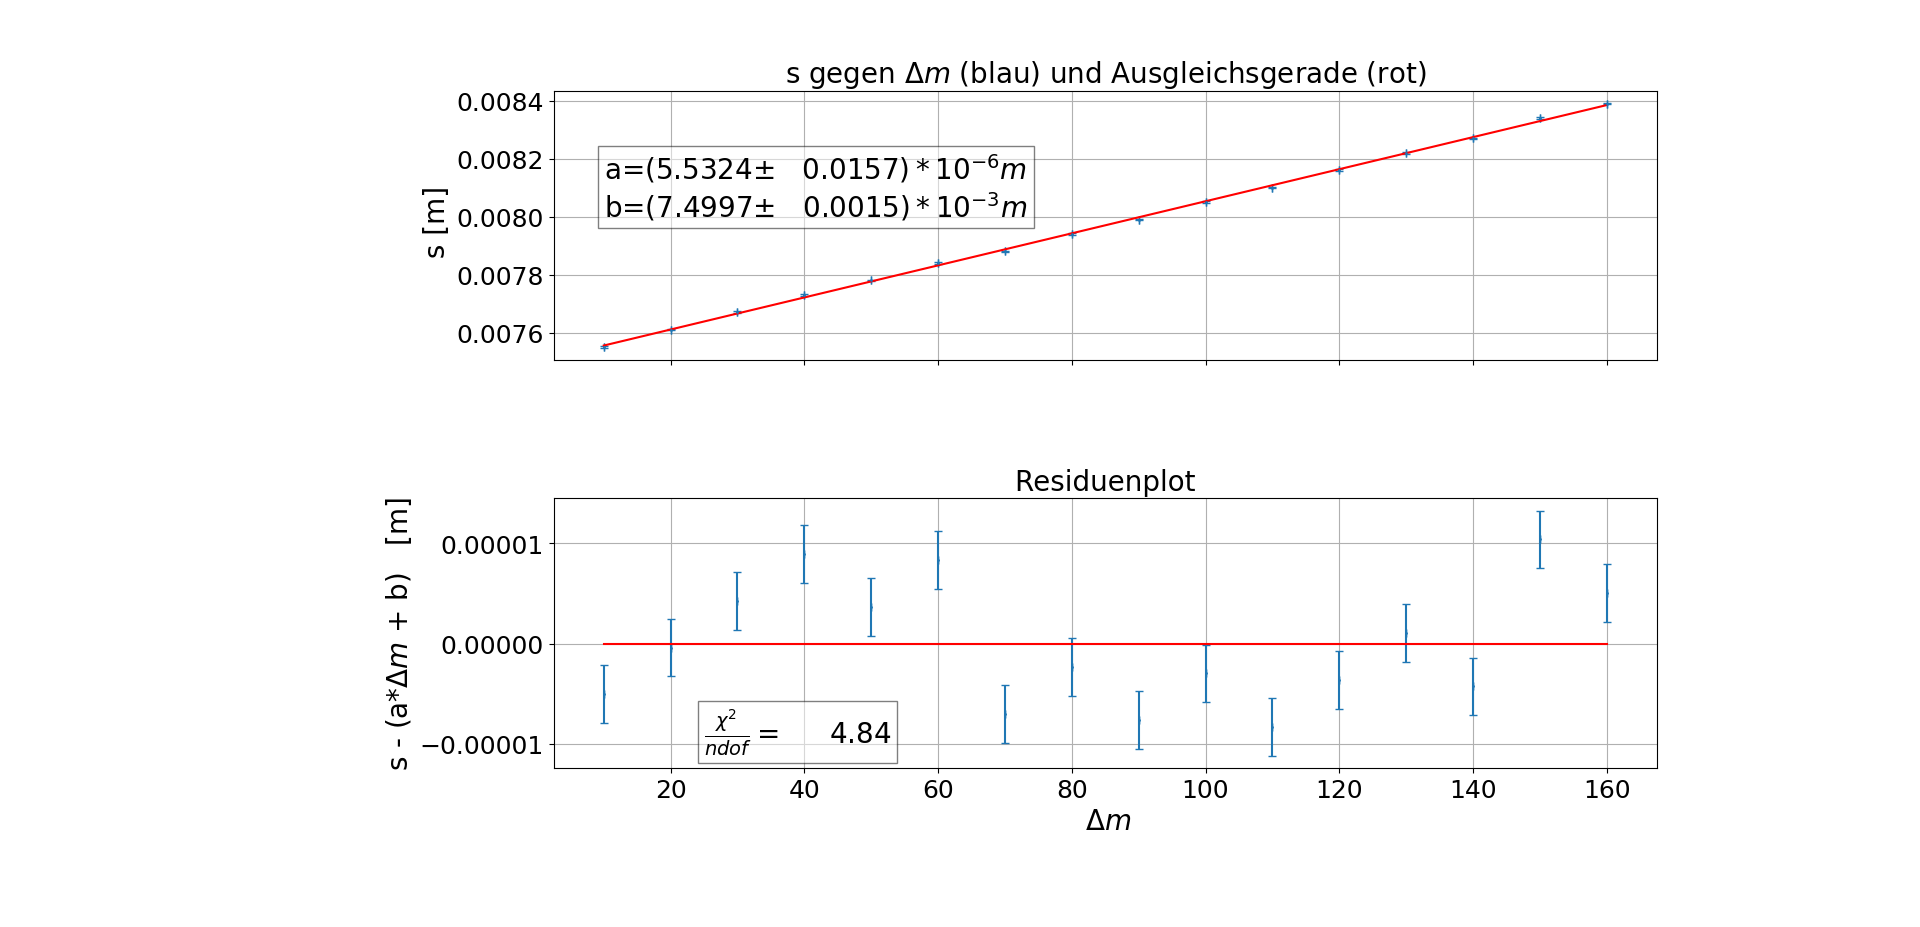
\includegraphics[trim={8cm 1cm 1cm 1cm},clip=true,width=1.1\linewidth]{./Bilder/Wellenlaengenbestimmung_1.png}
	\caption{Lineare Regression zur Bestimmung der Wellenlänge des grünen Lasers - Gruppe 1}
	\label{pic:lambda_1}	
\end{figure}

\begin{figure}[H]
	\centering
	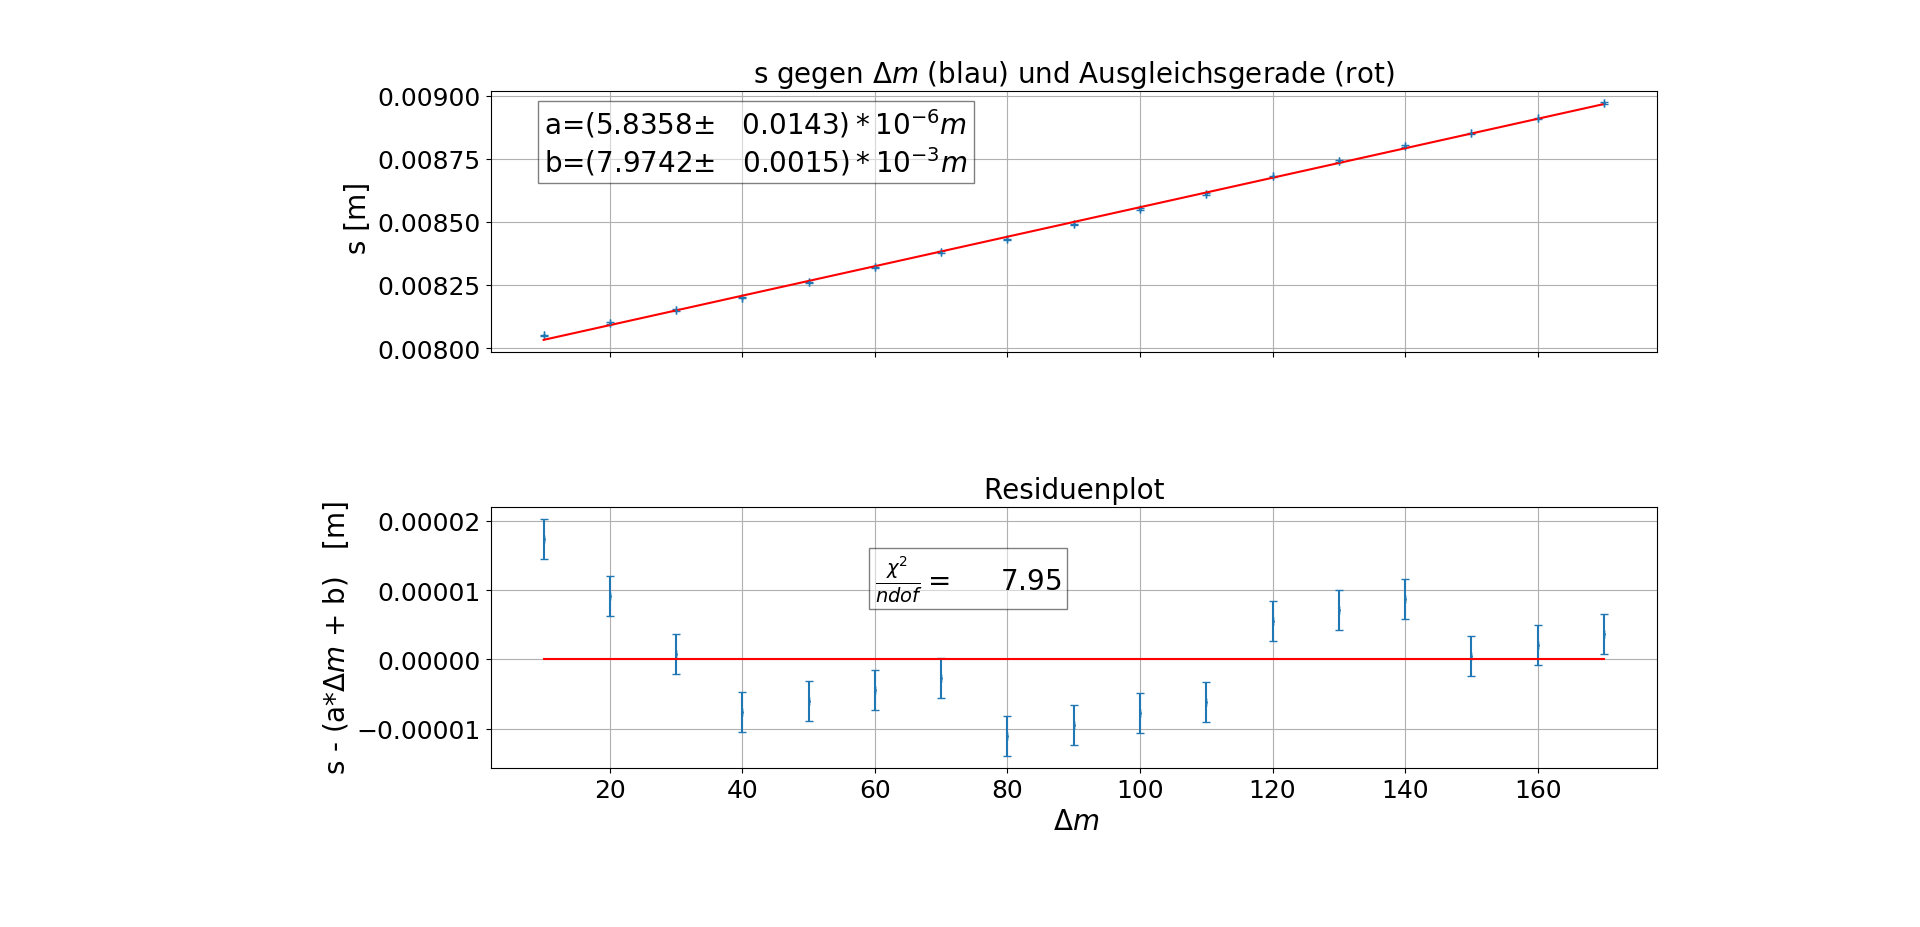
\includegraphics[trim={8cm 1cm 1cm 1cm},clip=true,width=1.1\linewidth]{./Bilder/Wellenlaengenbestimmung_2.png}
	\caption{Lineare Regression zur Bestimmung der Wellenlänge des grünen Lasers - Gruppe 2}
	\label{pic:lambda_2}	
\end{figure}

Aus der Steigung erhält man dann über $\lambda = 2 k a$ die Wellenlänge. Die statistische Unsicherheit auf $\lambda$ ergibt sich aus der Steigung der linearen Regression zu $\sigma_{\lambda_{stat}} = 2k\sigma_a$. Die Unsicherheit auf k ist hier von systematischer Natur und pflanzt sich analog über $\lambda = 2a \sigma_k$ fort. Die Endergebnisse dieses Teilversuches sind in Tabelle \ref{table:lambda_final} zusammengefasst.

\begin{table}[H]
	\renewcommand{\arraystretch}{1.5}
	\centering
	\begin{tabular}{|c|c|c|}
		\hline  	&	Gruppe 1	&	Gruppe 2  	\\
		\hline	$a$ &	$ (5.532 \pm 0.016) \,\mu m$		&	$ (5.836 \pm 0.014)\, \mu m $ \\
		\hline  $b$	&	$ (7.4997 \pm 0.0015)\, mm$		&	$ (7.9742 \pm 0.0015)\, mm$ \\
		\hline $\frac{\chi^2}{ndof}$	&	$4.84$	&	$7.95$	\\
		\hline  $k$	&	$ 0.04866 \pm 0.00008 $		&	$ 0.04586 \pm 0.00011$ \\
		\hline $\lambda$	&	$ (538.4 \pm 1.5 \pm 0.9)\, nm$ &	$ (535.2 \pm 1.3 \pm 1.4)\, nm $ \\
		\hline Abweichung von $\lambda_{gruen} = 532 nm$	&	$ 3.7 \sigma $		&	$ 1.7 \sigma $	\\
		\hline
	\end{tabular}
	\caption{Ergebnisse der Wellenlängenmessung des grünen Lasers}
	\label{table:lambda_final}
\end{table}

\subsection{Fazit}
Man erkennt, dass sowohl bei den Regressionen zur Kalibration, als auch bei denen zur eigentlichen Bestimmung der Wellenlänge der Fit nicht ideal geklappt hat und das $\frac{\chi^2}{ndof}$ in allen Fällen überhöht ist. In den meisten Fällen zeigt das Residuum eher eine statistische Schwankung, lediglich bei der Wellenlängenregression der 2. Gruppe erkennt man eine leichte Wannenform, die darauf schließen lässt, dass dort kein exakt linearer Zusammenhang besteht (diese lässt sich auch im Residuum der entsprechenden Kalibration erahnen, dies scheint aber eher statistischer Natur zu sein). Vor allem der Beginn des Bereiches fällt hier auf, so dass die Skalenübersetzung vielleicht in diesem Bereich nicht genau linear ist.

Bei allen Residuen fällt zudem auf, dass die Unsicherheiten der Messwerte wohl zu gering abgeschätzt wurden und wohl die als fehlerfrei angenommenen Zählungen nicht ganz exakt sind. Es könnte sein, dass durch Erschütterungen im Raum Interferenzordnungsänderungen übersehen oder doppelt gezählt wurden.

Dennoch liegen die eigentlichen Ergebnisse für die Wellenlängen mit Abweichungen von $3.7 \sigma$ bzw. $1.7 \sigma$ nicht allzu weit vom erwarteten Wert $\lambda_{gruen} = 532 \, nm$ entfernt.



\clearpage
\section{Druckabhängigkeit des Brechungsindex von Luft}
\subsection{Grundlagen}
Um das Verhalten des Brechungsindex von Luft in Abhängigkeit zum aktuellen Druck $P$ zu beschreiben, nimmt man eine lineare Näherung in Form einer Taylorentwicklung um den Punkt $P_0 = 0$ an
\begin{equation}
n(P) = n ( P_0 = 0) + \frac{\Delta n}{\Delta P}\cdot P = 1 + \frac{\Delta n}{\Delta P} \cdot P
\end{equation}
wobei man quadratische und höhere Ordnungen von $\frac{\Delta n}{\Delta P}$ vernachlässigt.

Man verwendet in diesem Versuchsteil eine Glasparzelle der Länge $L=10$mm (die vom Hersteller sehr genau bestimmt ist), in der nach und nach der Druck verringert werden soll. Durch Änderungen $\Delta n$ des Brechungsindex in der Glasparzelle ändert sich (mit zweifachem Durchlauf) der Glasparzelle die optische Weglängendifferenz zwischen den beiden Strahlengängen um 
\begin{equation}
m \cdot \lambda = \Delta d = 2L \Delta n
\end{equation}
Dabei ist m die Anzahl der durchlaufenen Maxima bzw. Minima im Zentrum des Interferenzmusters und $\lambda$ die zuvor bestimmte Wellenlänge des grünen Lasers. 
Damit erhält man als Zusammenhang für die Steigung die linearen Näherung: 
\begin{equation}
\frac{\Delta n}{\Delta P} = \frac{m}{\Delta P} \cdot \frac{\lambda}{2L}
\end{equation}

\subsection{Aufbau}
Man verwendet den selben Grundlegenden Aufbau wie im vorangegangenen Versuchsteil. Zusätzlich wird eine Glasparzelle in einen der Strahlengänge eingebaut, an die über ein T-Stück eine Handpumpe, sowie ein Druckmessgerät angeschlossen werden. Es muss darauf geachtet werden, dass im Aufbau kein Leck vorhanden ist, da sonst später keine genaue Druckmessung möglich ist.

\begin{figure}[H]
	\centering
	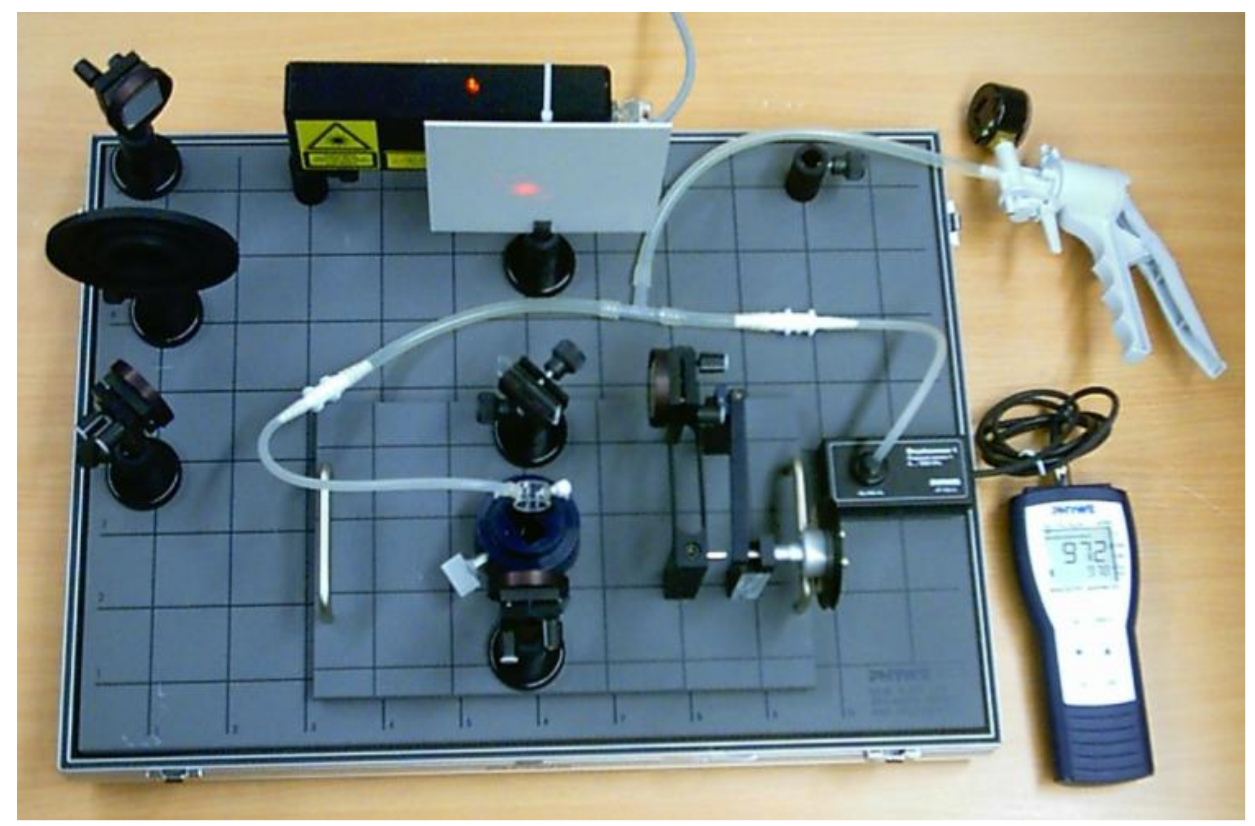
\includegraphics[scale=0.45]{./Bilder/Aufbau_Bild_Luft.png}
	\caption{Michelson-Interferometer mit eingebauter Glasparzelle}
	\label{pic:Aufbau_Bild_Luft}	
\end{figure}

\subsection{Durchführung}
Das Einfügen der Glasparzelle sollte auf den Strahlengang und damit auch auf das Interferenzbild eigentlich keinen Einfluss haben. Da es jedoch beim Einbau teils zu leichten Verschiebungen der Bauteile kommen kann, muss man gegebenenfalls die Spiegel ein wenig nachjustieren, um ein gut erkennbares Interferenzbild zu erhalten.

Für die eigentliche Messung notiert man zunächst die Normaldruckwerte, die das Druckmessgerät für den Außendruck und für den Druck innerhalb der Glasparzelle angibt. Dabei zeigte das Messgerät für den Außendruck konstant $P_0=992\mathrm{hPa}$ an. Die Daten des Messgeräts wurden zusätzlich noch mit der RWTH-Wetterstation Hörn \footnote{\url{http://www.klimageo.rwth-aachen.de/wtst/ACHoern.htm}} abgeglichen, welche zum Zeitpunkt des Versuchs einen Druck von $996\mathrm{hPa}$ angab. Somit waren die Daten des verwendeten Messgeräts realistisch.
 
Die Mikrometerschraube verstellt man zu Beginn so, dass das Interferenzbild im Zentrum ein klar erkennbares Maximum (oder Minimum) aufweist, und diese sich am Anfang des zuvor ausgemessenen linearen Bereichs befindet (siehe Tabelle \ref{table:lin_Bereich}), da sonst die Kalibration nicht mehr gewährleistet ist.
Danach verringert man mit der Handpumpe den Druck soweit, bis im Zentrum ein neues Maximum (oder Minimum) erscheint und notiert den in der Glasparzelle gemessenen Druckwert. Dies führt man so lange fort, bis man ca $ 100 \mathrm{hPa}$ als Druck erreicht oder der zum Pumpen notwendige Kraftaufwand zu groß wird (im Falle der Verwendung einer Handpumpe aus  Plastik).

Der gesamte Messvorgang wird insgesamt 8 mal durchgeführt, um später statistische Unsicherheiten auf die Druckmessungen abschätzen zu können.

\subsection{Auswertung}
\begin{figure}[H]
	\centering
	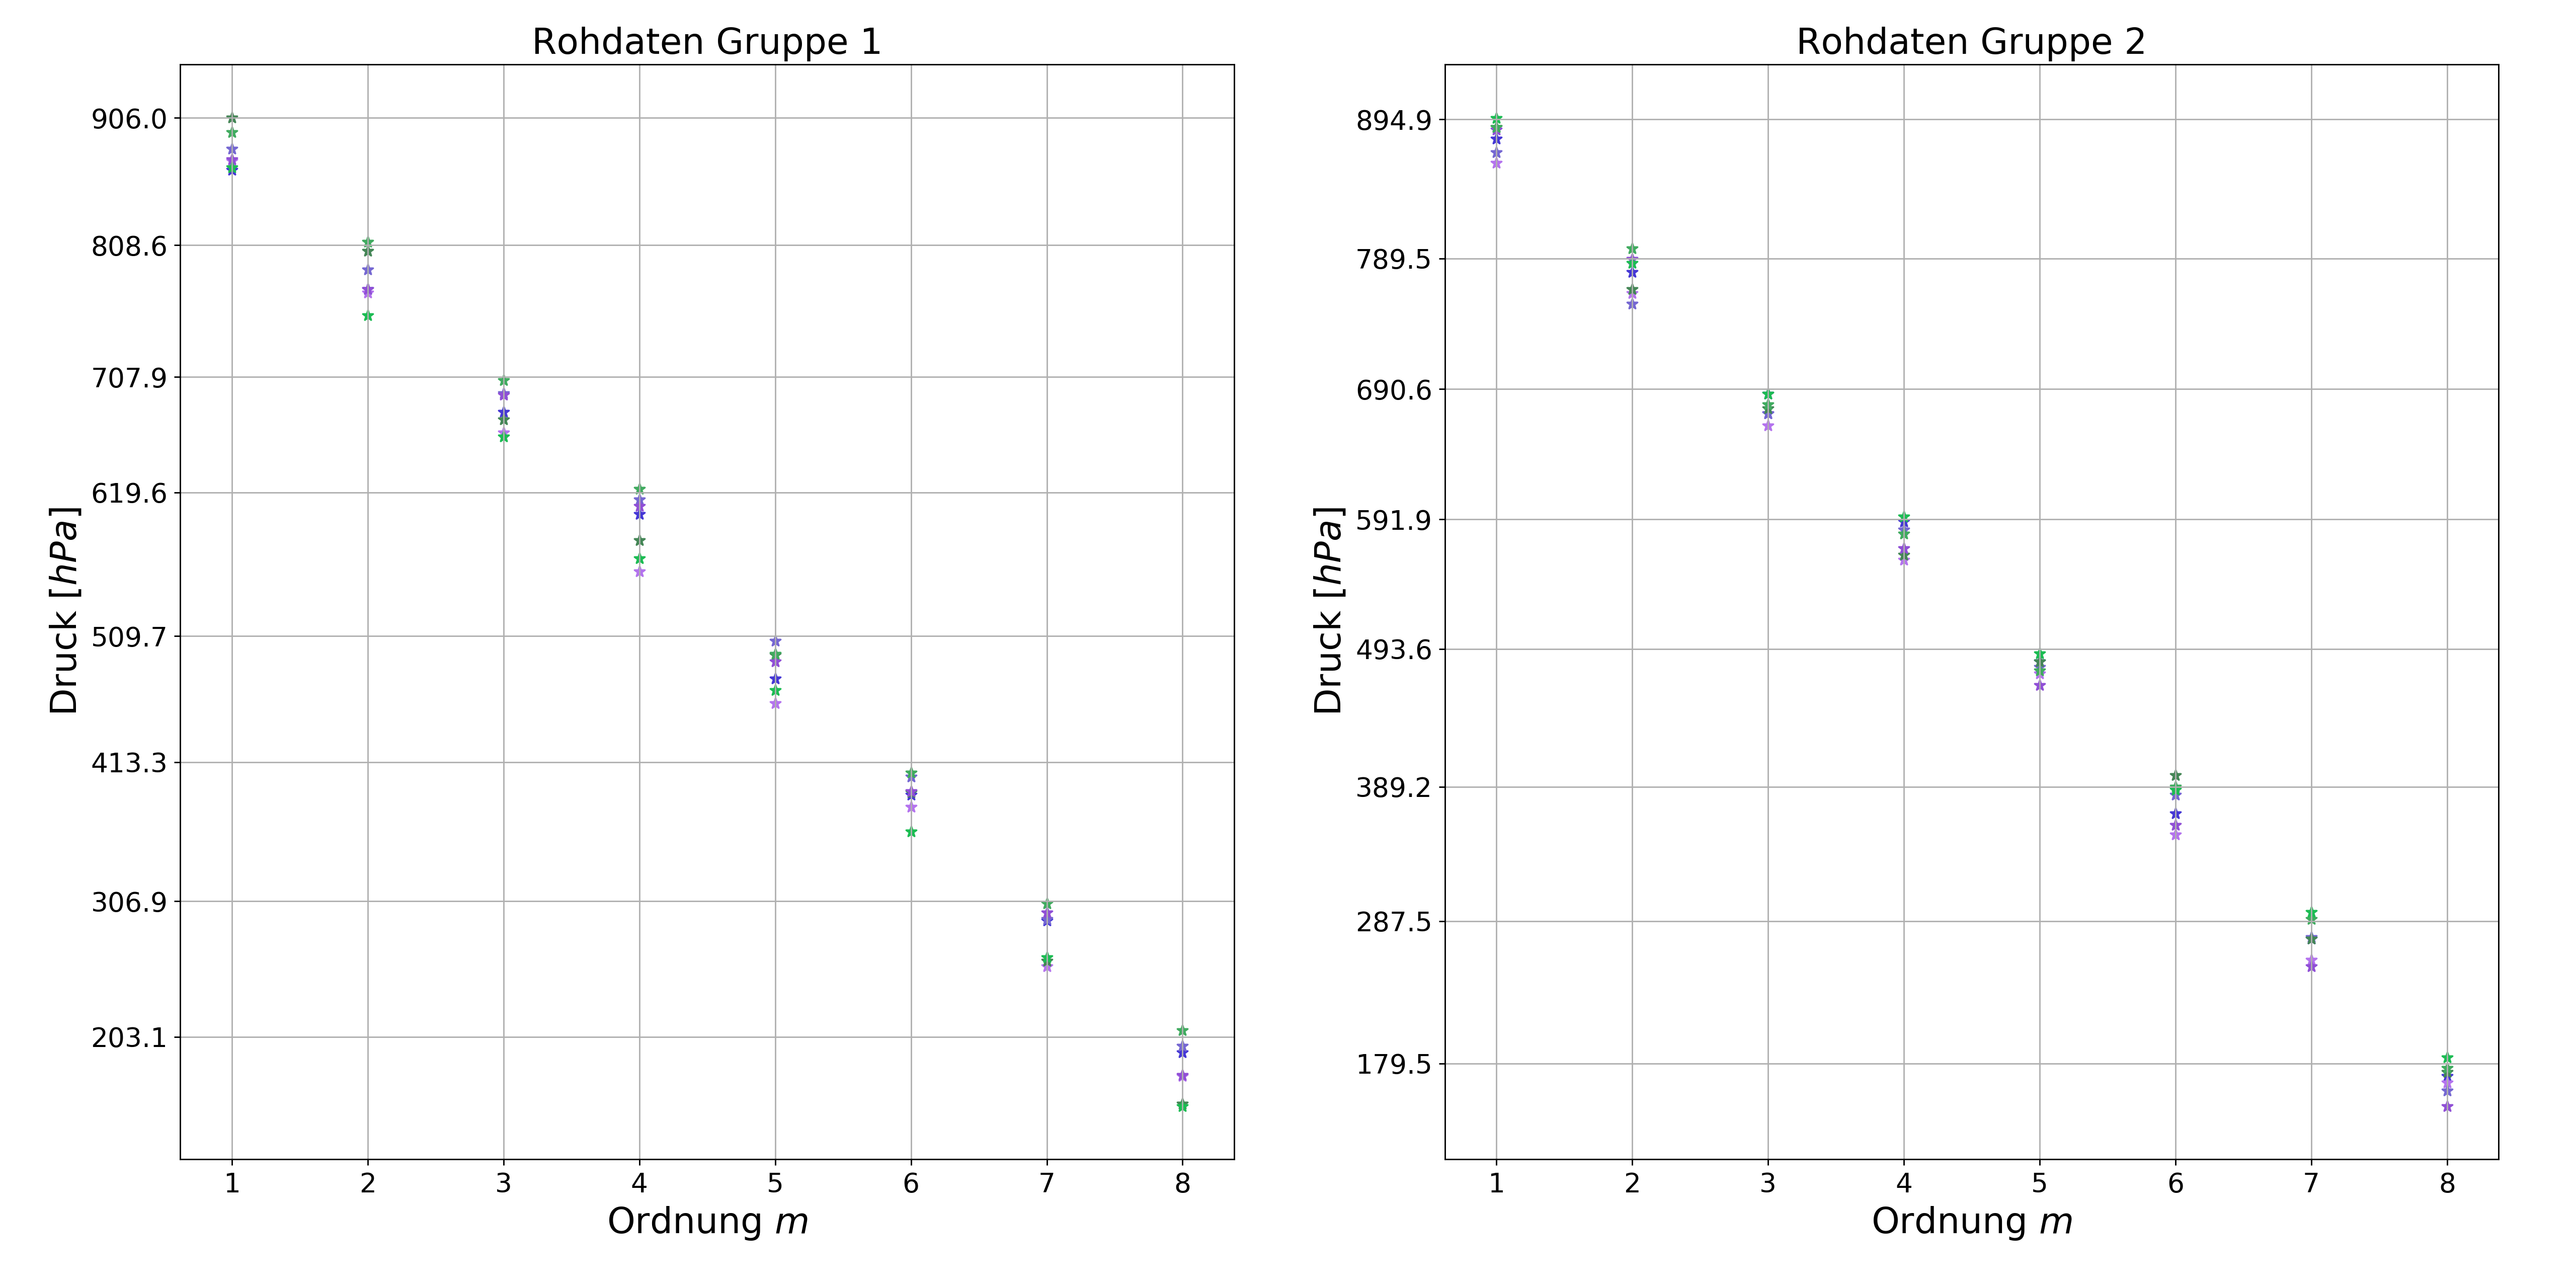
\includegraphics[scale=0.35]{./Bilder/Rohdaten.png}
	\caption{Rohdaten der Druckmessung}
	\label{pic:DruckmessungRoh}	
\end{figure}

Die gemessenen Werte für $\Delta P$ und $\Delta m$ werden nun gegeneinander aufgetragen, so dass sich als Steigung $a=\frac{1}{\frac{\Delta n}{\Delta P}} \cdot \frac{\lambda}{2L}$ ergibt. Bevor daran nun jedoch eine lineare Regression durchgeführt werden kann,  werden die einzelnen Punkte um den Abstand zum Maximalwert der ersten Messung verschoben, sodass die ersten Punkte der jeweiligen Messreihen zusammen fallen. Die dafür notwendige Verschiebung wird jeweils auf die gesamte Messreihe fortgesetzt, dadurch sollen systematische Verschiebungen korrigiert werden, da das Messziel lediglich die Steigung ist. Die Rohdaten sind in Abbildung \ref{pic:DruckmessungRoh} zu sehen, die verschobenen Daten mit Fehler befinden sich im Anhang (Abbildung \ref{pic:RohdatenShifted}).

Aus den Punkten für ein $m$ wird nun der Mittelwert und die Standardabweichung gebildet, daraus wird nun der Fehler auf den Mittelwert zu $\sigma_{\bar{x_i}}=\frac{\sigma_{x_i}}{\sqrt{n}}$ bestimmt. Da der erste Punkt ja so erzeugt wurde dass es dort keine Standardabweichung gibt, schätzen wir die Messunsicherheit dort als Mittelwert aller übrigen $\sigma_{\bar{x_i}}$ ab. Aus der linearen Regression folgt nun die Steigung mit Unsicherheit $\sigma_a$. Damit ergibt sich für die Druckabhängigkeit des Brechungsindex
\begin{equation}
\frac{\Delta n}{\Delta P}=\frac{1}{a}\frac{\lambda}{2L} 
\qquad
\sigma_{\frac{\Delta n}{\Delta P}} = \sqrt{\left(\frac{1}{a^2} \frac{\lambda}{2L}\right)^2 \cdot \sigma_a^2 + \left(\frac{1}{2L \cdot a}\right)^2 \cdot \sigma_{\lambda}^2}
\end{equation}

Aus den durchgeführten linearen Regressionen (Abbildungen \ref{pic:linReg1} und \ref{pic:linReg2}) ergaben sich die Werte in Tabelle \ref{table:linRegLuft}. Offensichtlich ist die Steigung der Ausgleichsgeraden negativ, was daher kommt dass $\Delta m$ positiv angenommen wurde, die Ringe im Interferenzbild aber vermutlich verschwanden und nicht hinzukamen. Für die Berechnung von $\Delta n/\Delta P$ wird natürlich ein positiver Wert verwendet.

Der zum Vergleich angenommene Literaturwert von $\Delta n/\Delta P = 2.665\cdot10^{-7} \, \mathrm{hPa}^{-1}$ wurde im Praktikumsskript für die Wellenlänge $\lambda_{rot} = 632,8$nm des roten Lasers angegeben, hier wurde aber ein grüner Laser verwendet. Eigentlich müsste man aufgrund von Dispersion einen Wert für $\lambda_{gruen}$ nehmen, es wurde jedoch mit Hilfe der Edlen-Gleichung \footnote{Hierbei wurde der durch \texttt{NIST} bereitgestellte Rechner verwendet: \url{http://emtoolbox.nist.gov/Wavelength/Edlen.asp}} festgestellt, dass dieser Effekt innerhalb unseres Druck- und Wellenlängenbereichs so klein ist, dass er weit unterhalb unserer Messungenauigkeit liegt.

\begin{table}[H]
	\renewcommand{\arraystretch}{1.5}
	\large
	\centering
	\begin{tabular}{|c|c|c|}
		\hline
		& Gruppe 1 & Gruppe 2 \\ 
		\hline
		$\lambda$ [nm] & $538.4 \pm1.5\pm0.9$ & $535.2 \pm1.3\pm1.4$  \\
		\hline
		Steigung a [hPa] & $-99.7 \pm 0.9$	& $-101.3 \pm 0.6$ \\
		\hline
		$\chi^2/ndf$ & $0.524$ & $0.799$ \\
		\hline
		$\Delta n/\Delta P \mathrm{[hPa^{-1}]}$ & $(2.701 \pm 0.024 \pm 0.009)\cdot10^{-7}	$ &	$(2.642 \pm 0.015 \pm 0.009)\cdot10^{-7}$	\\
		\hline
		Abweichung & $1.758\sigma$ & $0.741\sigma$\\
		\hline
	\end{tabular}
	\caption{Ergebnisse der linearen Regression zur Druckabhängigkeit von $n_{Luft}$}
	\label{table:linRegLuft}
\end{table}


\begin{figure}[H]
	\centering
	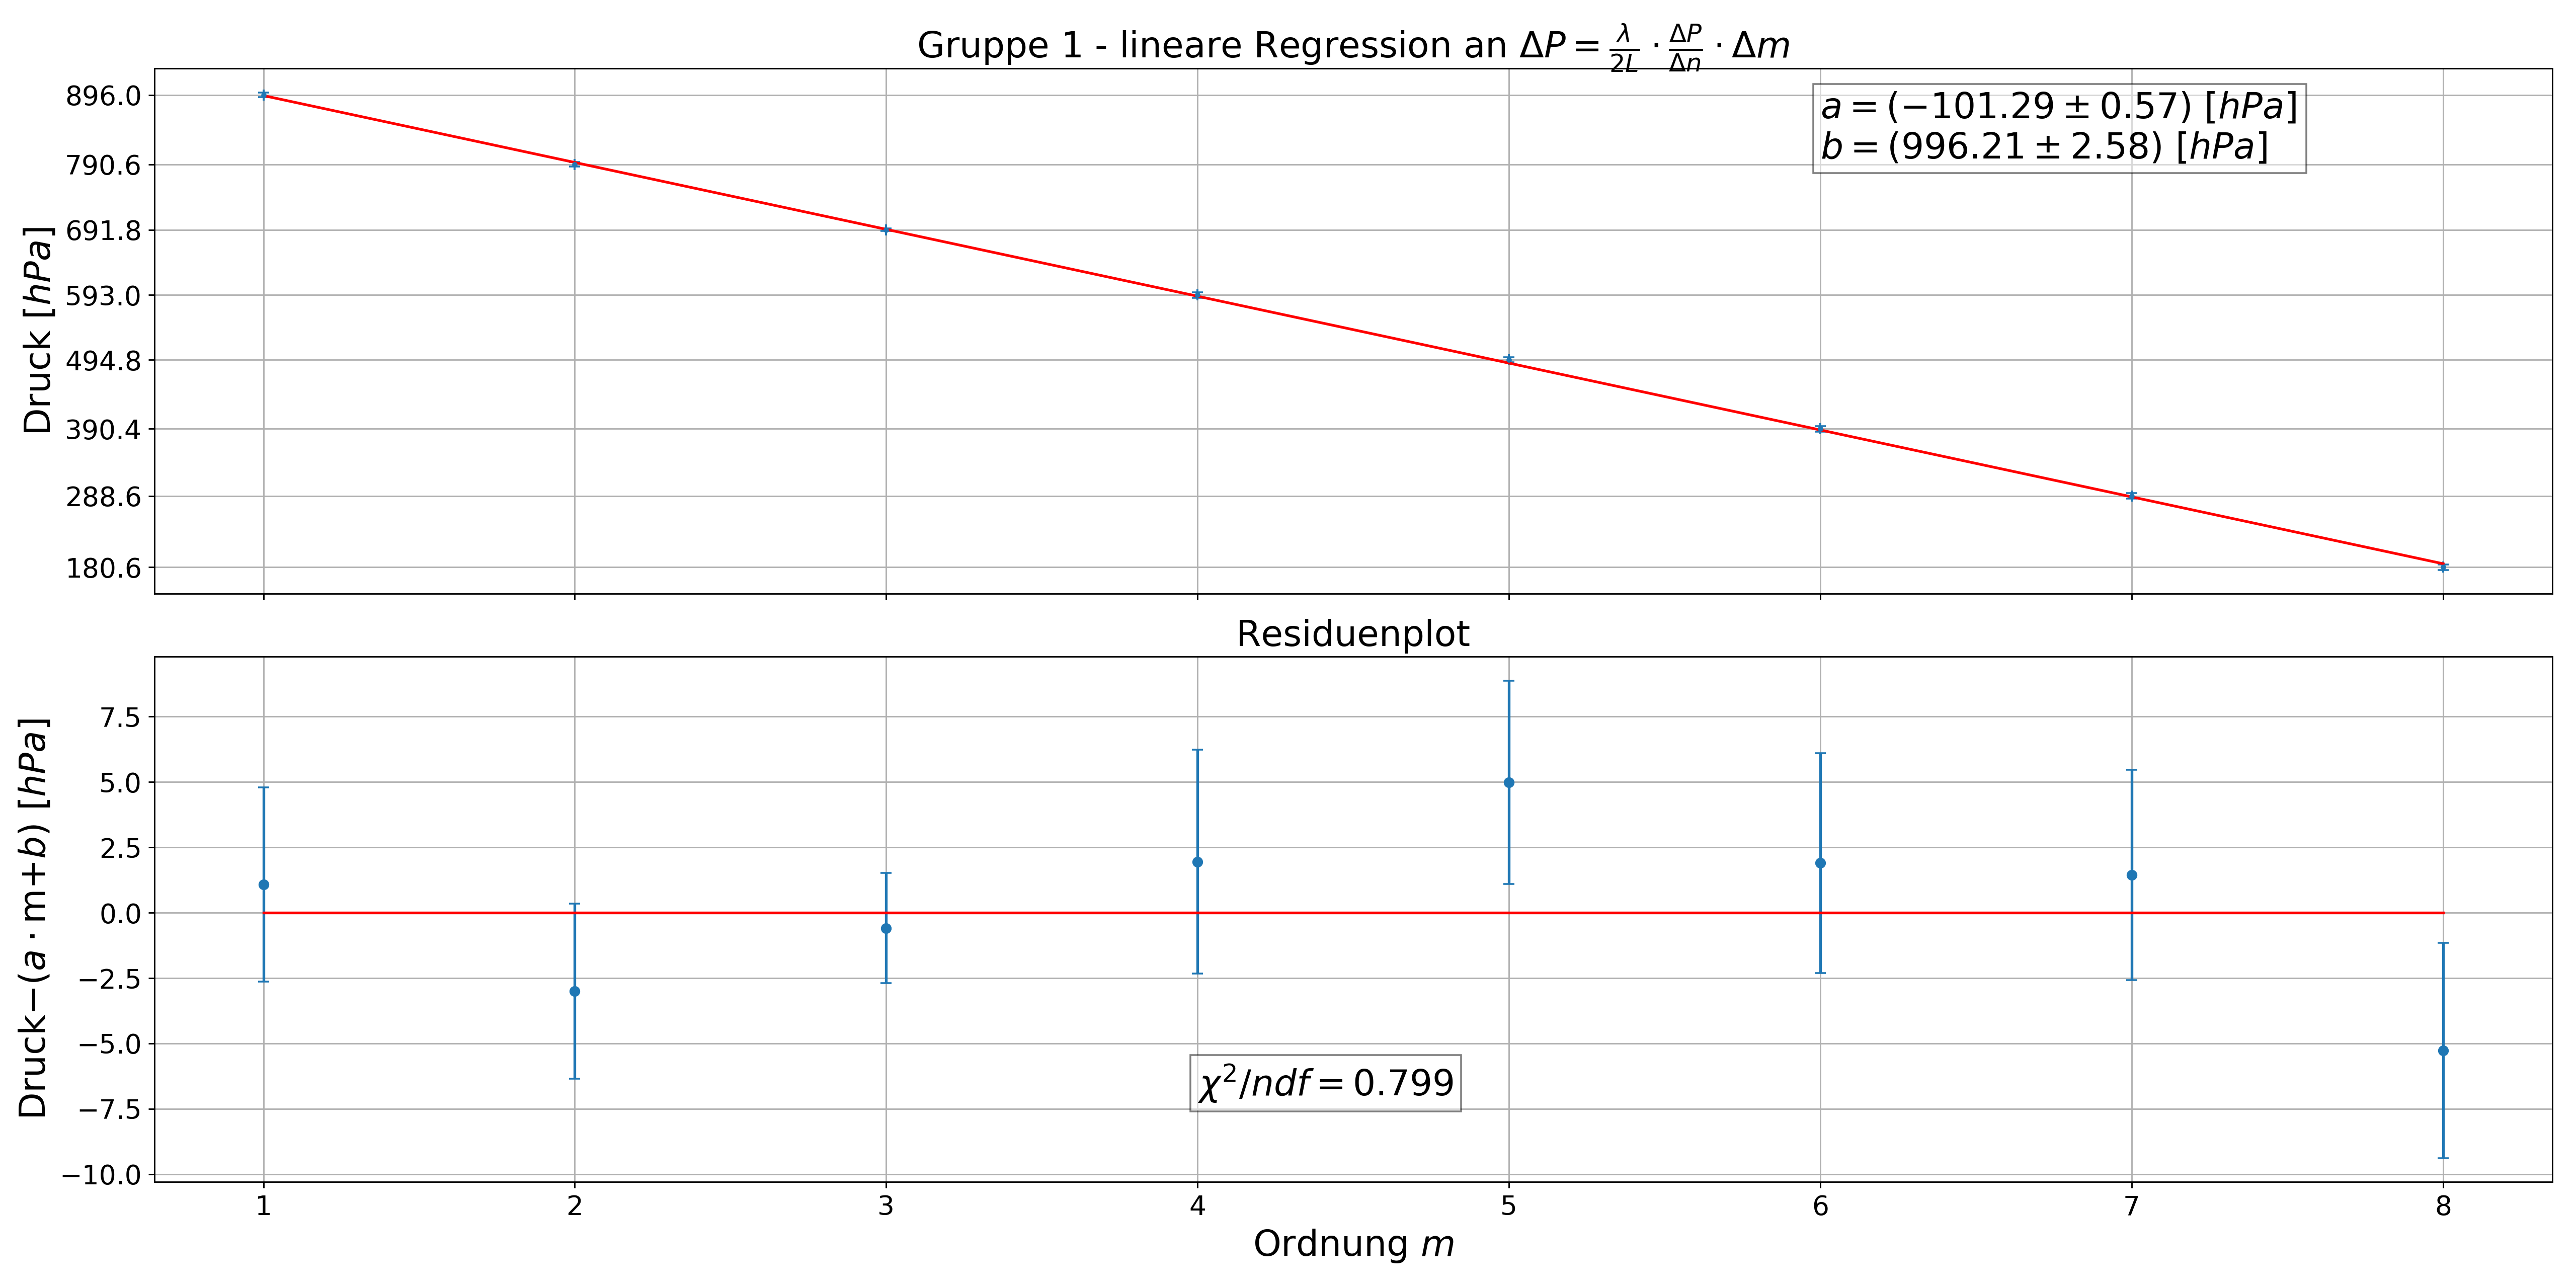
\includegraphics[scale=0.3]{./Bilder/Gruppe1_linReg.png}
	\caption{linearen Regression zur Druckabhängigkeit von $n_{\mathrm{Luft}}$ - Gruppe 1}
	\label{pic:linReg1}	
\end{figure}


\begin{figure}[H]
	\centering
	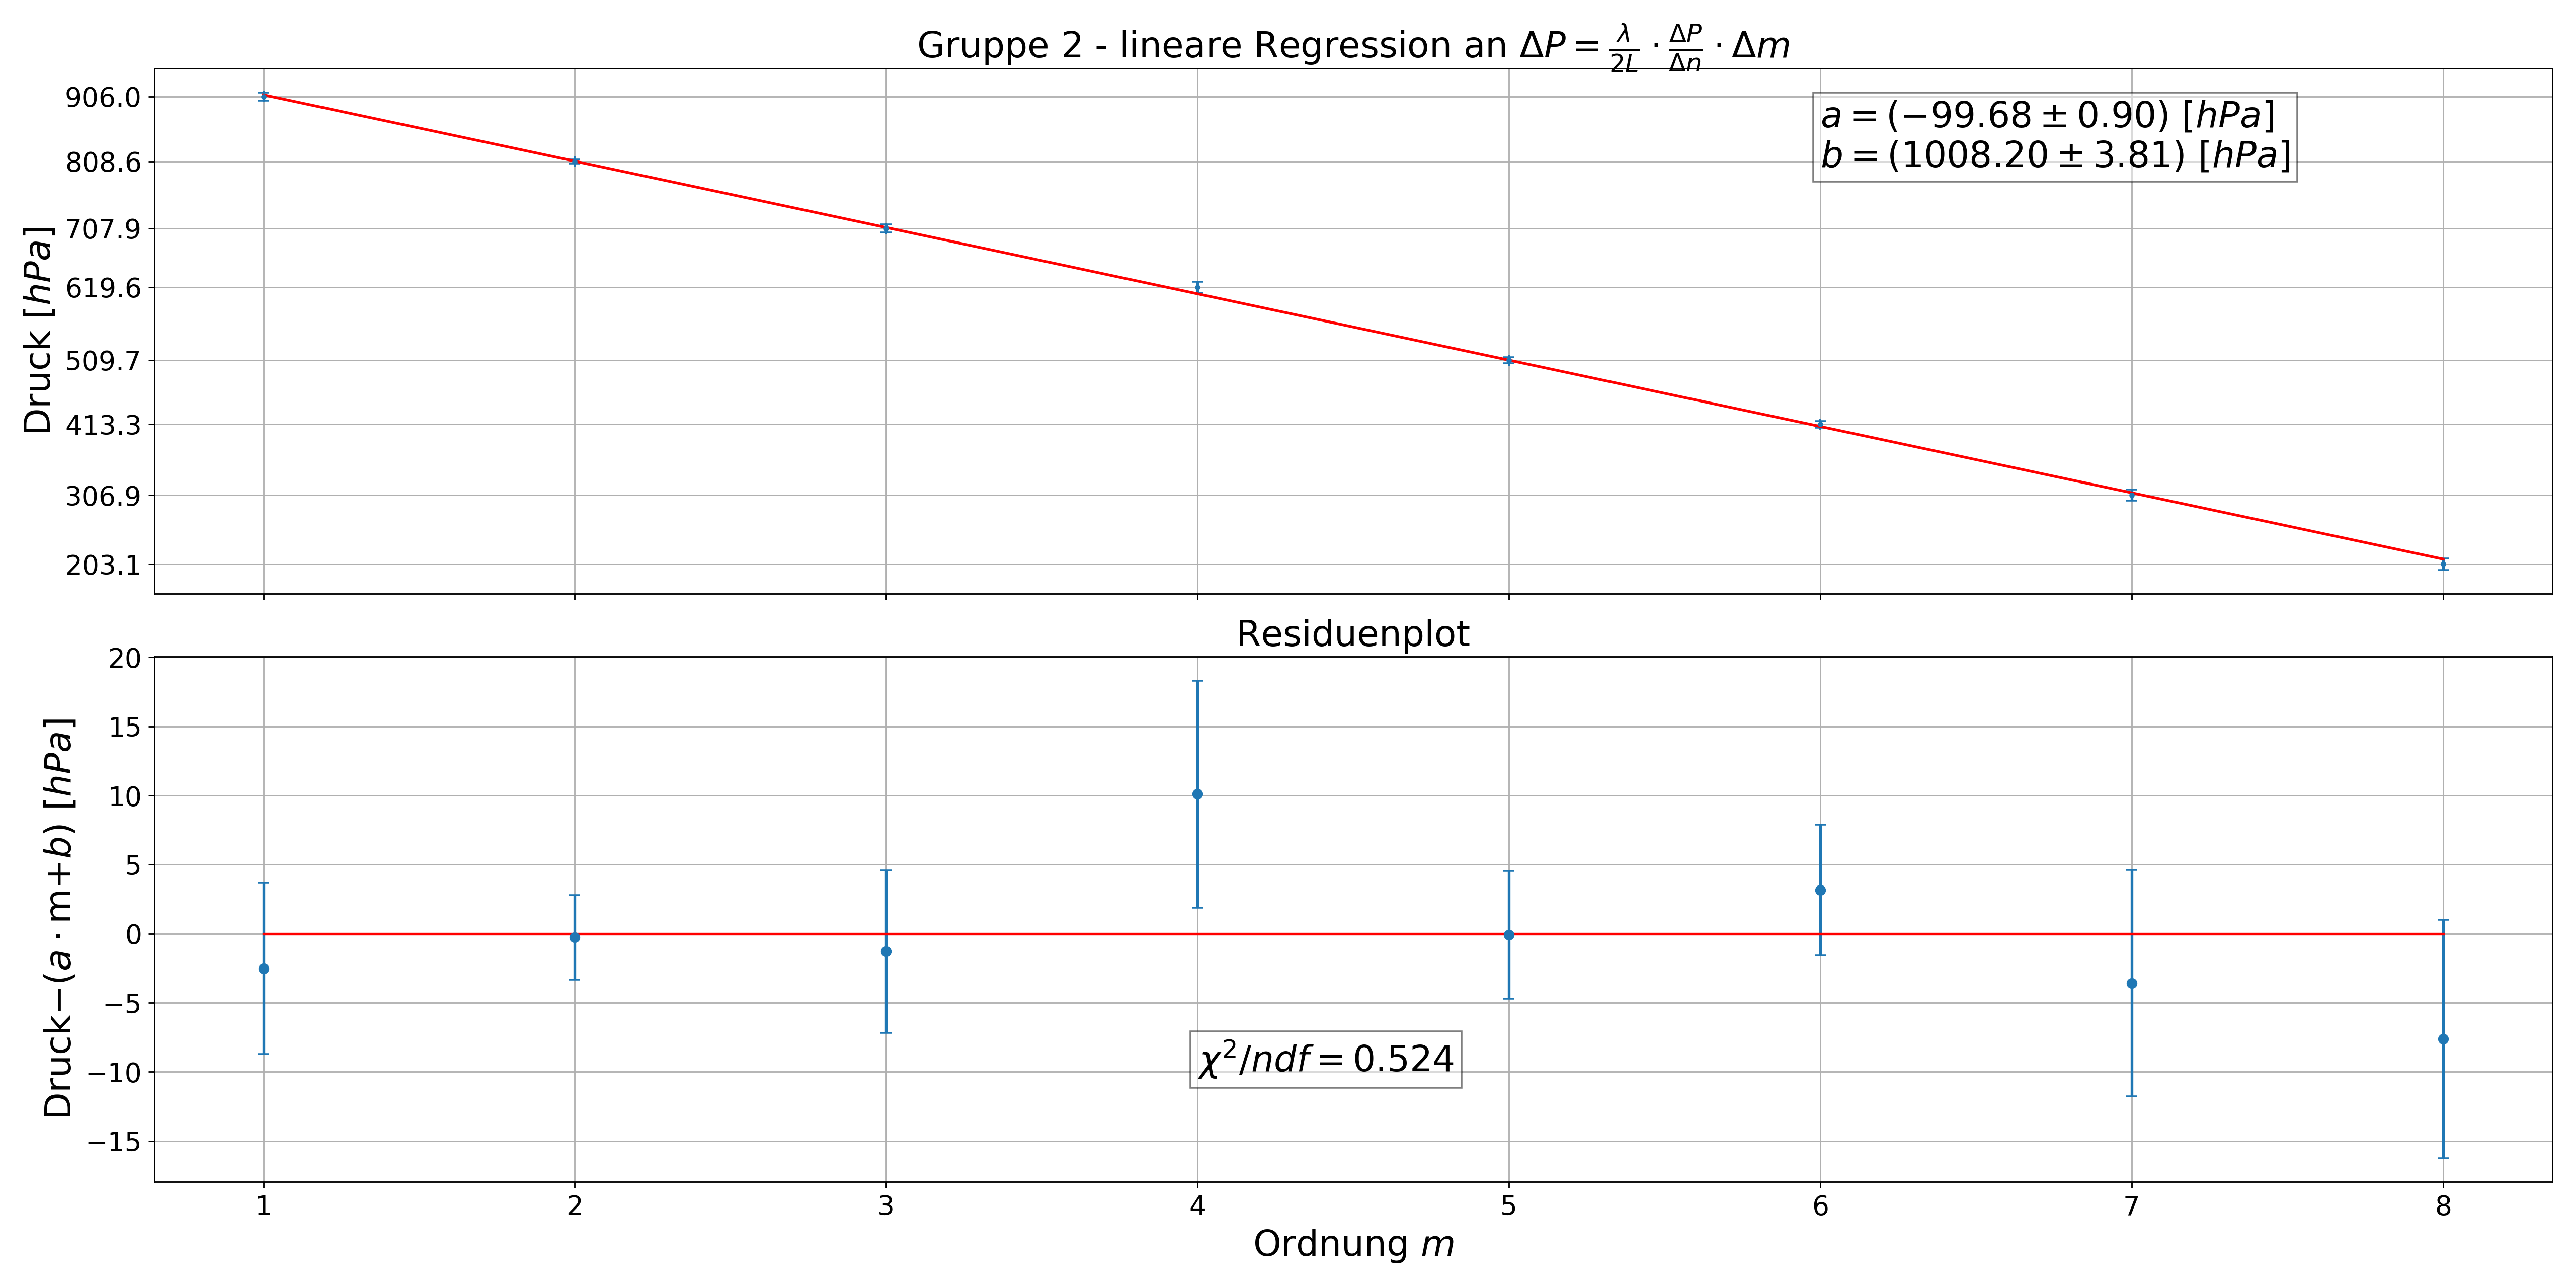
\includegraphics[scale=0.3]{./Bilder/Gruppe2_linReg.png}
	\caption{linearen Regression zur Druckabhängigkeit von $n_{\mathrm{Luft}}$ - Gruppe 2}
	\label{pic:linReg2}	
\end{figure}

\subsection{Fazit}
Anhand der Residuenplots (die keine Systematik aufweisen) erkennt man, dass durch die Methode der Verschiebung der Messwerte um den Abstand zum Maximalwert der ersten Messung relativ große Fehler auf den Druck zustande kamen, was auch zu einem $\chi^2/ndf \, < \, 1$ führte.

Trotz Schwierigkeiten bei der Zählung der Ringe und ungenauen Druckmessung (aufgrund von nicht vermeidbaren Lecks im System) lies sich die Druckabhängigkeit des Brechungsindex von Luft mit Abweichung von $0.7\sigma$ und $1.7\sigma$ vom Literaturwert recht gut messen.

\clearpage
\section{Brechungsindex Kohlenstoffdioxid}
\subsection{Grundlagen}
Für diesen Teilversuch wird der Aufbau im Vergleich zum Versuch mit Luft nicht verändert, lediglich die Glasparzelle wird an einer Öffnung offen gelassen und an der anderen wird eine $\mathrm{CO_2}$ Gasflasche angeschlossen. Des weiteren kann diesmal noch eine Kamera verwendet werden um den Schirm aufzunehmen. Da die Brechungsindizes von Luft und $\mathrm{CO_2}$ unterschiedlich sind, sorgt der Gasaustausch in der Parzelle für eine zusätzliche Differenz in der optischen Weglänge
\begin{equation}
\Delta d=2\cdot (n_{\mathrm{CO_2}}-n_{\mathrm{Luft}}) \cdot L\end{equation}
wobei L hier die Dicke der Parzelle bezeichnet. Die Parzelle wird wieder zweimal durchlaufen.
Mit der bereits bekannten Bedingung für Maxima folgt
\begin{equation}
\Delta d= \lambda \cdot \Delta m
\quad \Rightarrow \quad 
n_{\mathrm{CO_2}}-n_{\mathrm{Luft}}=\Delta n= \Delta m \frac{\lambda}{2L}
\end{equation}
Also lässt sich bei bekanntem Brechungsindex für Luft der für $\mathrm{CO_2}$ berechnen.

\subsection{Durchführung}
Da $\mathrm{CO_2}$ eine höhere Dichte als Luft hat, sinkt das Gas nach unten und verdrängt die Luft so lange das offene Ventil oberhalb liegt. Solange also Luft verdrängt wird ändert sich das Interferenzbild, sobald keine Änderung mehr stattfindet ist die Luft komplett verdrängt und die Messung somit beendet. Man sollte bei der Befüllung der Glasparzelle über eine $\mathrm{CO_2}$-Flasche darauf achten, dass man diese möglichst vorsichtig öffnet, damit die Änderung im Interferenzbild nachher noch gut erkennbar ist. Anhand der Videoaufnahme lassen sich jetzt die durchlaufenen Minima und Maxima abzählen, daraus und aus der im ersten Teilversuch bestimmten Wellenlänge folgt dann $n_{\mathrm{CO_2}}$.

\subsection{Auswertung}
Wir haben 7 Videos aufgenommen von denen nur 3 brauchbar waren, die anderen 4 waren entweder zu unscharf, um etwas erkennen zu können oder das Ventil der $\mathrm{CO_2}$-Flasche wurde zu schnell geöffnet, so dass die Interferenzringe sich zu schnell veränderten. Somit wurde nur die Videos 1,5 und 6 ausgewertet. Bei jedem Video wurden mehrfach von verschiedenen Teammitgliedern die Ordnungsübergänge gezählt und dann gemittelt, was in Tabelle \ref{table:VideosMaxima} zu sehen ist.

Aus jedem dieser drei Mittelwerte wurde mit Hilfe von \eqref{eq:DeltaN} ein $\Delta n$ bestimmt.
\begin{eqnarray}\label{eq:DeltaN}
\Delta n=\Delta m \cdot \frac{\lambda}{2L} &
\sigma_{stat}=\frac{\lambda}{2L}\cdot \sigma_{\Delta m} &
\sigma_{sys}=\frac{\Delta m}{2L}\cdot \sigma_{\lambda} 
\end{eqnarray}

\newcommand*\mean[1]{\overline{#1}}
\begin{table}[H]
\centering
\renewcommand{\arraystretch}{1.5}
%\large
\begin{tabular}{|c|c|c|c|}
	\hline 
	Video & 1 & 5 & 6 \\
	\hline 
	$\Delta m$ &5 & 4.5 & 4.25 \\
	&5.25& 4.25 &4.5 \\
	& 5.5&5&4 \\
	& 5.5&4.75&4.25 \\
	& 5&4.75&4.5 \\
	&5&4.75&4.5 \\
	\hline 
	$\mean{\Delta m}$ & $5.21 \pm 0.13$&$4.67 \pm 0.14$&$4.33 \pm 0.11$ \\
	\hline
	$\Delta n$ & $(1.394 \pm 0.025 \pm 0.005  )\cdot10^{-4}$ & $(1.271 \pm 0.04 \pm 0.005 )\cdot10^{-4}$ & $(1.182 \pm 0.04 \pm 0.005 )\cdot10^{-4}$ \\
	\hline
\end{tabular}
\caption{In den Videos gezählte Ordnungsübergänge (Mehrfachzählungen)}
\label{table:VideosMaxima}
\end{table}

Da die Werte innerhalb ihrer Fehlern nicht übereinstimmen, wird für das gewichtete Mittel an Stelle des inneren, der äußere Fehler verwendet:
\begin{equation*}
\Delta n=(1.28 \pm 0.05)\cdot10^{-4}
\end{equation*}

Um mit dem Im Skript gegebenen Literaturwert zu vergleichen berechnen wir:
\begin{equation}
n_{\mathrm{CO_2}}-1=\Delta n + n_{Luft}-1
\end{equation}

Mit dem gemessenen Außendruck von $P_0=992\mathrm{hPa}$ und den Ergebnissen der linearen Regression ergibt sich ein Brechungsindex von Luft bei Normaldruck von $n_{\mathrm{Luft}}=1.0002636 \pm 0.0000018$.
Damit ergibt sich für den Brechungsindex von $\mathrm{CO_2}$:

\begin{table}[H]
\centering
	\begin{tabular}{|c|c|c|c|}
	\hline 
	& Literaturwert & berechneter Wert & Abweichung \\
	\hline 
	$n_{CO_2}-1$ & $4.16\cdot 10^{-4}$ & $(3.92\pm0.06)\cdot 10^{-4}$ & $4.5 \sigma$ \\
	\hline
	\end{tabular}
\caption{Ergebnisse für den Brechungsindex von $\mathrm{CO_2}$ }
\label{table:nCO2Ergebnis}
\end{table}

\subsection{Fazit}
Bei diesem Versuch war das Problem, dass die Videos fast alle unbrauchbar waren, sodass nur wenige Daten zur Verfügung standen. Die Daten sind somit sehr fehleranfällig und mit einer Abweichung von 4.5 $\sigma$ konnte der Literaturwert nur schlecht bestätigt werden. Bei einer hypothetischen erneuten Versuchsdurchführung sollte dieser Versuchsteil also genauer durchgeführt und insbesondere der Fluss des $\mathrm{CO_2}$ besser kontrolliert werden.


\clearpage
\section{Anhang}
\begin{figure}[H]
	\centering
	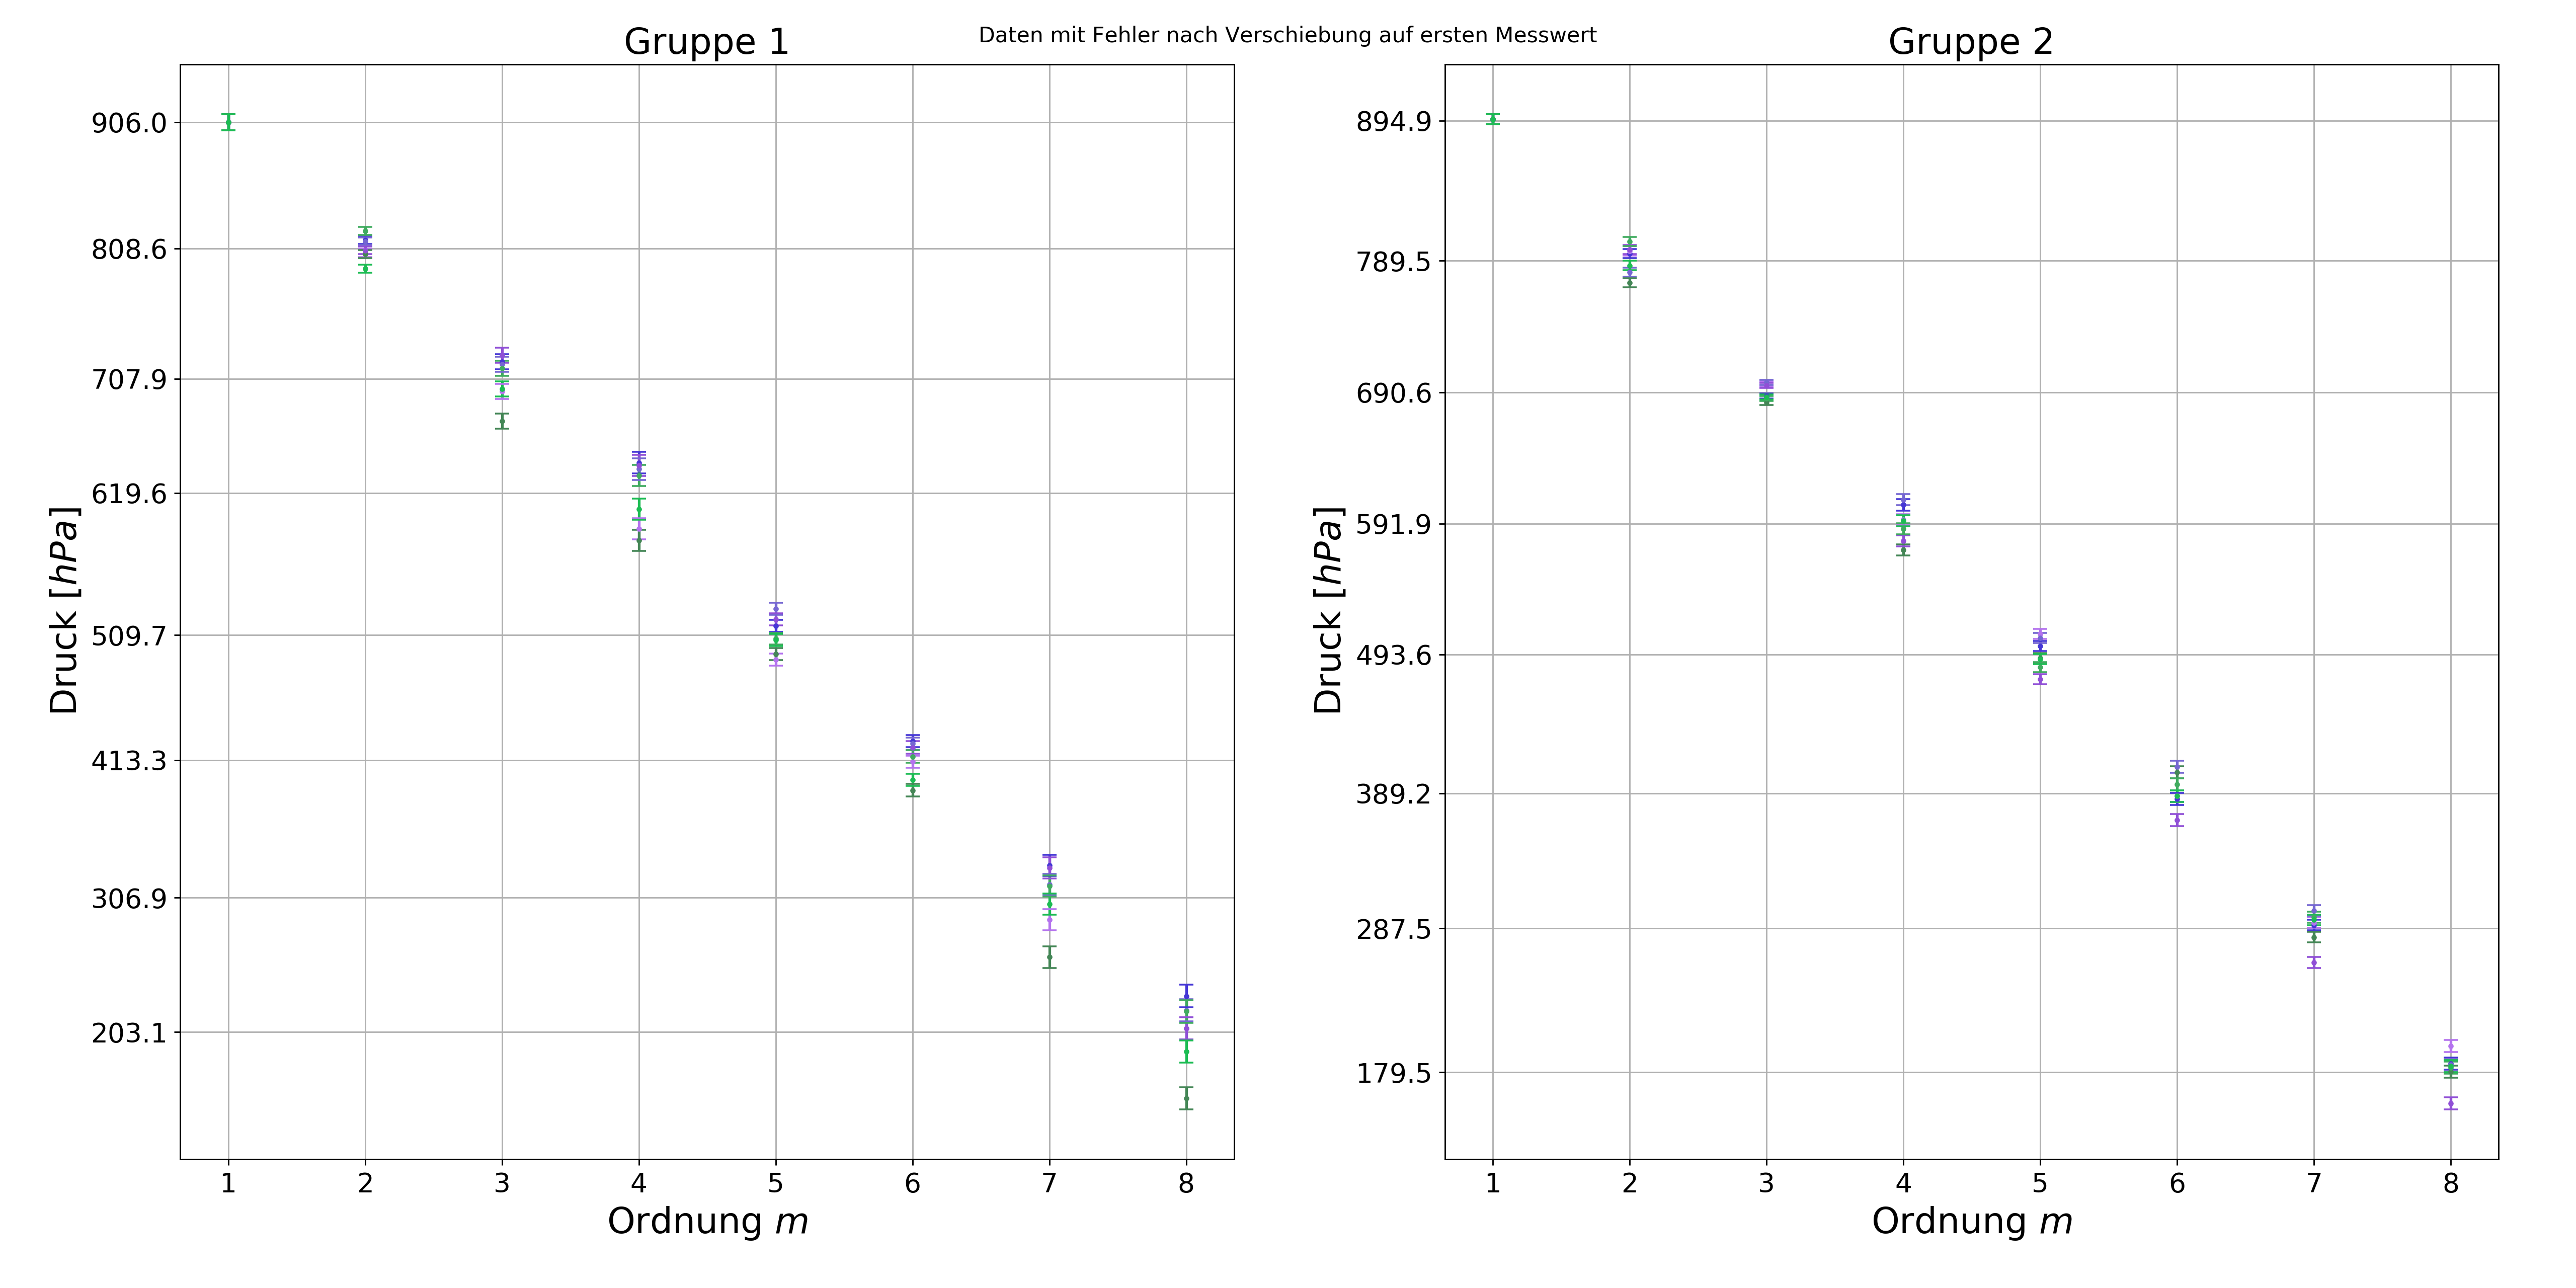
\includegraphics[scale=0.35]{./Bilder/DatenShifted.png}
	\caption{Daten der Druckmessung, Verschoben um den Abstand zum ersten Messwert der jeweiligen Reihe}
	\label{pic:RohdatenShifted}	
\end{figure}

\clearpage
\listoffigures
\listoftables

\end{document}
